\documentclass[german]{spicker}

%\addbibresource{dbv.bib}

\title{Digitale Bildverarbeitung}
\subtitle{Sommersemester 2023}
\university{Fachhochschule Aachen}
\programme{Angewandte Mathematik und Informatik, M. Sc.}
\lecturer{Prof. Dr.-Ing. Klaus Drechsler}

\author{Patrick Gustav Blaneck}

\makeindex[intoc]
\makeindex[intoc, name=Beispiele,title=Beispiele]

% Declare custom units
\DeclareSIUnit{\ppi}{ppi}
\DeclareSIUnit{\ppc}{ppc}
\DeclareSIUnit{\pixel}{Pixel}

% Declare custom operators
\DeclareMathOperator{\high}{high}
\DeclareMathOperator{\low}{low}
\DeclareMathOperator{\height}{height}
\DeclareMathOperator{\width}{width}

\begin{document}
\maketitle
\tableofcontents
\disclaimer


% Until 06/25/2023
% \section{Einleitung}

\begin{defi}{Digitale Bildverarbeitung}
    \emph{Digitale Bildverarbeitung} ist das Entwerfen, Entwickeln und/oder Erweitern von Software oder Algorithmen zur Verarbeitung von Bildern mit einem Digitalrechner.

    Dagegen steht die Bildbearbeitung, die das (interaktive) Bearbeiten von Bildern mit Hilfe von Software wie Adobe Photoshop oder GIMP bezeichnet.
\end{defi}

\begin{bonus}[Digitale Bildverarbeitung]{Verwandte Gebiete}
    Verwandte Gebiete zur digitalen Bildverarbeitung sind z. B.:
    \begin{itemize}
        \item \emph{Computergrafik}: Erzeugung von Bildern aus geometrischen Modellen
        \item \emph{Signalverarbeitung}: Verarbeitung von Signalen (z.B. Audio, Video, Sprache, etc.)
        \item \emph{Augmented Reality}: Fusionierung realer und virtueller Bilder
        \item \emph{Virtual Realiity}: Erzeugung von virtuellen Welten
        \item \emph{Algorithmische Geometrie}: Algorithmen und Datenstrukturen zur Verarbeitung geometrischer Objekte
    \end{itemize}

    Generell lassen sich die Gebiete unter dem Oberbegriff \emph{Visual Computing} zusammenfassen.
\end{bonus}

\begin{bonus}[Digitale Bildverarbeitung]{Anwendungsgebiete}
    Digitale Bildverarbeitung kommt z. B. in folgenden Bereichen zum Einsatz:
    \begin{itemize}
        \item \emph{Aufbereitung von Bildmaterial}: z. B. Rauschunterdrückung, Kontrastanpassung, Farbkorrektur, etc.
        \item \emph{Fusionierung von Animationen mit realem Filmmaterial}: z. B. in der Filmindustrie
        \item \emph{Medizinische Bildverarbeitung}: z. B. zur Erkennung von Tumoren, Bestrahlungsplanung, etc.
        \item \emph{Astronomie}: z. B. zur Erkennung von Objekten im Weltall
        \item \emph{Automobilindustrie}: z. B. zur Erkennung von Verkehrszeichen, Fahrspuren, etc.
    \end{itemize}
\end{bonus}

 % VL 01
% \section{Bildaufnahme}

\begin{defi}[Kamera]{Schema}

    \centering
    \includegraphics[width=0.8\textwidth]{figures/kamera-schema.pdf}
\end{defi}

\begin{defi}[Kamera]{Filter}
    % TODO: https://de.wikipedia.org/wiki/Filter_(Fotografie) 
    \emph{Filter} sind optische Elemente eines bildgebenden Systems, die in der Fotografie meist vor dem Objektiv der Kamera angebracht werden.

    Sie verändern das einfallende Licht bereits vor dem Objektiv und Film oder Bildsensor.
    Sie werden verwendet, um optische Effekte positiv zu korrigieren oder spezielle Effekte zu erreichen.

    Während optische Filter vor der Erfindung der Digitalfotografie ein wichtiges Element der analogen Fotografie waren, spielen sie mittlerweile durch immer bessere Kamerasoftware und spätere Bearbeitungsmöglichkeiten eine zunehmend geringere Rolle -- mit wenigen Ausnahmen wie etwa Polfiltern und Neutraldichtefiltern.
\end{defi}

\begin{example}[Kamera]{Filter}
    % TODO: https://de.wikipedia.org/wiki/Filter_(Fotografie) 
    Die meisten Filter reflektieren einen Teil des einfallenden Lichtes, so dass weniger Licht das Objektiv erreicht.
    Diese Belichtungsreduktion wird durch den Filterfaktor angegeben.
    Dieser ist meist auf der Fassung des Filters angegeben.

    Wichtige Filter sind z. B.:
    \begin{itemize}
        \item \emph{Polarisationsfilter}
        \item \emph{UV-Sperrfilter} und Skylightfilter
        \item \emph{Farbfilter} bzw. \emph{Konversionsfilter} und \emph[Korrekturfilter] (Rot, Grün, Blau, Gelb etc.)
        \item \emph{optische Spezialfilter}
        \item \emph{Infrarot-Sperrfilter}
        \item \emph{Neutraldichtefilter} (kurz ND-Filter, meist auch als Graufilter bezeichnet)
        \item \emph{Effektfilter} (z. B. Stern-, Regenbogen- und Farbverlauffilter)
    \end{itemize}
\end{example}

\begin{defi}[Kamera]{Objektiv}
    % TODO: https://de.wikipedia.org/wiki/Objektiv_(Optik) 
    Ein \emph{Objektiv} ist ein sammelndes optisches System, das eine reelle optische Abbildung eines Gegenstandes (Objektes) erzeugt. Es ist die wichtigste Komponente abbildender optischer Geräte, zum Beispiel von Kameras, Ferngläsern, Mikroskopen, Projektoren oder astronomischen Teleskopen.

    Das einfachste Objektiv ist eine einzelne Sammellinse, wie sie um 1608 die ersten Fernrohre hatten.
    Bestandteile eines Objektivs können jedoch sowohl Linsen, als auch Spiegel oder (seltener) Beugungsgitter sein, die sich je nach Einsatzzweck in einem oder mehreren Tuben befinden, die innen geschwärzt und gerippt sind, um Streulicht zu reduzieren.

    Die Hauptmerkmale eines Objektivs sind dessen Brennweite, die für einen gegebenen Objektabstand den Abbildungsmaßstab bestimmt, und die Apertur (freie Öffnung der Frontlinse).

    Weitere wichtige Eigenschaften sind die Abbildungsqualität, die durch eine geeignete Kombination mehrerer Linsen unterschiedlicher Brechungsindizes, Dicken und Krümmungsradien bestimmt wird und zur Verringerung optischer Abbildungsfehler dient, sowie die Streulichtempfindlichkeit, die möglichst gering sein sollte.
    Die Streulichtempfindlichkeit ist vor allem bei Gegenlicht wichtig und kann durch geschwärzte Blenden vermindert werden.

    Weitere Eigenschaften sind die fotografische Lichtstärke (Öffnungsverhältnis) und die Naheinstellgrenze, welche bestimmt, wie nah man an das Motiv \enquote{herangehen} kann (Makro).
\end{defi}

\begin{defi}[Kamera]{Linse}
    Als \emph{Linsen} bezeichnet man in der Optik transparente Scheiben, von deren zwei Oberflächen wenigstens eine -- meistens sphärisch -- gekrümmt ist.

    Durchgehendes Licht wird an den Oberflächen gebrochen und zur Mitte des Lichtbündels abgelenkt (gesammelt, Sammellinse) oder nach außen gestreut (Zerstreuungslinse).
    Eine konvexe Oberfläche sammelt, eine konkave Oberfläche zerstreut das Licht.

    Die Größe des Bildes wird von der \emph{Brennweite} $f$ der Linse und dem Abstand $g$ zwischen Gegenstand und Linse bestimmt.

    \centering
    % TODO: https://de.wikipedia.org/wiki/Linsengleichung 
    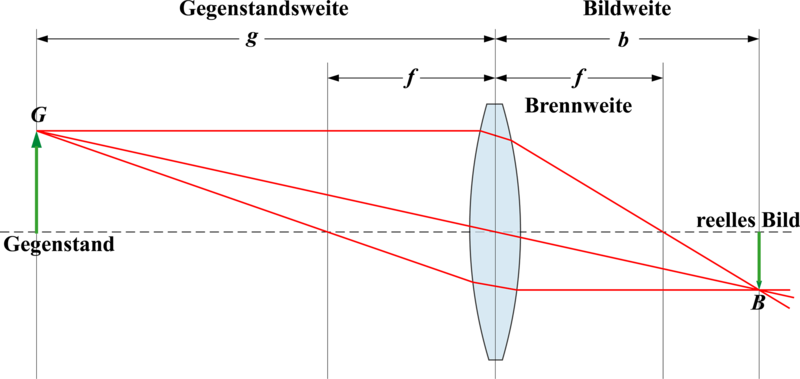
\includegraphics[width=0.6\textwidth]{figures/linse.png}
\end{defi}

\begin{defi}{Abbildungsmaßstab}
    % TODO: https://de.wikipedia.org/wiki/Abbildungsmaßstab 
    Der \emph{Abbildungsmaßstab} $\beta$ ist definiert als das Verhältnis zwischen der Bildgröße $B$ der optischen Abbildung eines Gegenstandes und dessen realer Objektgröße $G$.
    Alternativ kann der Abbildungsmaßstab auch über das Verhältnis von Bildweite $b$ zur Gegenstandsweite $g$ bestimmt werden:
    \[
        \beta = \frac{B}{G} = \frac{b}{g}
    \]
\end{defi}

\begin{defi}{Linsengleichung}
    % TODO: https://de.wikipedia.org/wiki/Linsengleichung 
    Die \emph{Linsengleichung} gibt bei einer optischen Abbildung mittels einer Linse die Beziehung zwischen Gegenstandsweite $g$, Bildweite $b$ und Brennweite $f$ an.
    Sie lautet:
    \[
        \frac{1}{f} = \frac{1}{b} + \frac{1}{g}
    \]
\end{defi}

\begin{defi}[Kamera]{Blende}
    % TODO: https://de.wikipedia.org/wiki/Blende_(Optik) 
    \emph{Blenden} sind in der Optik Vorrichtungen, die den Querschnitt von Strahlenbündeln begrenzen.

    Eine reine \emph{Aperturblende} beeinflusst die Helligkeit des Bildes gleichmäßig, indem sie die Öffnungsweite (Apertur) des optischen Geräts begrenzt.
    Sie wirkt sich nicht auf die Größe des Bildausschnitts aus.
    Dazu muss sie so beschaffen sein, dass alle Strahlenbündel bezogen auf die Strahlungsleistung des Objekts den gleichen Strahlungsfluss enthalten.

    In der Praxis führt nahezu jegliche Begrenzung eines Strahlenbündels durch eine Aperturblende dazu, dass ein Strahlenbündel, das den Blendenquerschnitt in einem anderen Winkel passiert, in einem anderen Verhältnis beschnitten wird.
    Das führt zu einer Verdunkelung des Bildes in Randnähe.
\end{defi}

\begin{defi}{Lichtstärke}
    % TODO: https://de.wikipedia.org/wiki/Lichtst%C3%A4rke_(Fotografie)
    Die \emph{fotografische Lichtstärke} ist ein Maß für das Vermögen eines Objektivs, für eine optische Abbildung Licht zu sammeln.

    Sie kann als Zahlenwert durch das maximale Öffnungsverhältnis $V_{\max}$ angegeben werden.
    Dabei stehen kleinere Zahlenwerte für eine größere Eintrittsöffnung des Objektivs und damit für höhere Lichtstärke.

    Die Lichtstärke ist neben der Brennweite der wichtigste Kennwert eines Objektivs in der Fotografie, beide werden in der Regel zusammen angegeben.

    Bei vielen abbildenden optischen Geräten kann das Öffnungsverhältnis aus dem Durchmesser der Eintrittspupille (der Apertur) $D$ und der Brennweite $f$ gebildet werden, wobei sich das maximale Öffnungsverhältnis bei vorgegebener Brennweite durch den fest vorgegebenen oder maximal einstellbaren Durchmesser der Eintrittspupille $D_{\max}$ ergibt:
    \[
        V_{\max} = \frac{D_{\max}}{f}
    \]
\end{defi}


\begin{defi}{Blendenzahl}
    % TODO: https://de.wikipedia.org/wiki/Lichtst%C3%A4rke_(Fotografie)
    % TODO: https://de.wikipedia.org/wiki/Blendenreihe_(Optik) 
    Der Kehrwert der Lichtstärke ist die ebenfalls dimensionslose \emph{Blendenzahl} $k$:
    \[
        k = \frac{1}{V_{\max}} = \frac{f}{D_{\max}}
    \]

    Die \emph{Blendenreihe} ist so angelegt, dass die durch das Objektiv fallende Lichtmenge sich von Blendenstufe zu Blendenstufe
    \begin{itemize}
        \item halbiert, wenn die nächste Blendenstufe einen höheren Wert hat (beispielsweise 11 $\to$ 16) oder
        \item verdoppelt, wenn die nächste Blendenstufe einen kleineren Wert hat (beispielsweise 11 $\to$ 8).
    \end{itemize}

    Der Blendendurchmesser $D$ vergrößert bzw. verkleinert sich von Blendenstufe zu Blendenstufe um den Faktor $\sqrt{2}$ bzw. $\frac{1}{\sqrt{2}}$, wodurch sich Fläche und Lichtmenge verdoppeln bzw. halbieren.
    Diese Abstufung entspricht der üblichen Belichtungszeitreihe und ermöglicht dadurch ein einfaches Anpassen von Blende und Belichtungszeit bei gegebener Beleuchtung.

    Jede Blendenzahl $k$ wird aus der vorhergehenden durch Multiplikation mit $\sqrt{2}$ berechnet.
    Demnach lässt sich eine beliebige Blendenstufe durch die Formel $k=({\sqrt{2}})^{{(n-1)}}$ mit $n=1,2,3,\dots$ errechnen.

    Normalerweise wird die Blendenzahl auf eine oder zwei Stellen abgerundet angegeben, so dass sich die folgende Reihe ergibt:

    \centering
    \begin{tabular}{c|ccccccccccccccc}
        \toprule
        $n$   & 1 & 2   & 3 & 4   & 5 & 6   & 7 & 8  & 9  & 10 & 11 & 12 & 13 & 14 & 15  \\
        \midrule
        $k_n$ & 1 & 1,4 & 2 & 2,8 & 4 & 5,6 & 8 & 11 & 16 & 22 & 32 & 45 & 64 & 90 & 128 \\
        \bottomrule
    \end{tabular}
\end{defi}

\begin{defi}{Schärfentiefe}
    % TODO: https://de.wikipedia.org/wiki/Sch%C3%A4rfentiefe 
    Die \emph{Schärfentiefe} ist ein Maß für die Ausdehnung des scharfen Bereichs im Objektraum eines abbildenden optischen Systems.
    Sie beschreibt die Größe des Entfernungsbereichs, innerhalb dessen ein Objekt hinlänglich scharf abgebildet wird.

    In der Regel wird eine große Schärfentiefe durch kleine Blendenöffnungen oder Objektive mit kurzen Brennweiten erreicht;
    von vorn bis hinten sieht dann alles mehr oder weniger scharf aus.

    Die Schärfentiefe wird außer durch die Wahl der Brennweite und der Entfernungseinstellung auch durch die Blendenöffnung beeinflusst:
    je größer die Blendenöffnung (kleine Blendenzahl), umso geringer ist die Schärfentiefe.
    Bei einer Entfernungseinstellung (Fokussierung) auf ein nahes Objekt ist der optisch als scharf erfasste Objektraum \enquote{von-bis} kürzer als bei einer Fokussierung auf ein weiter entferntes Objekt.

    Die Wahl der Blendenöffnung ist Teil der Belichtungseinstellung.

    Nur eine Ebene, die \emph{Schärfeebene}, parallel zum Sensor, ist scharf.

    \centering
    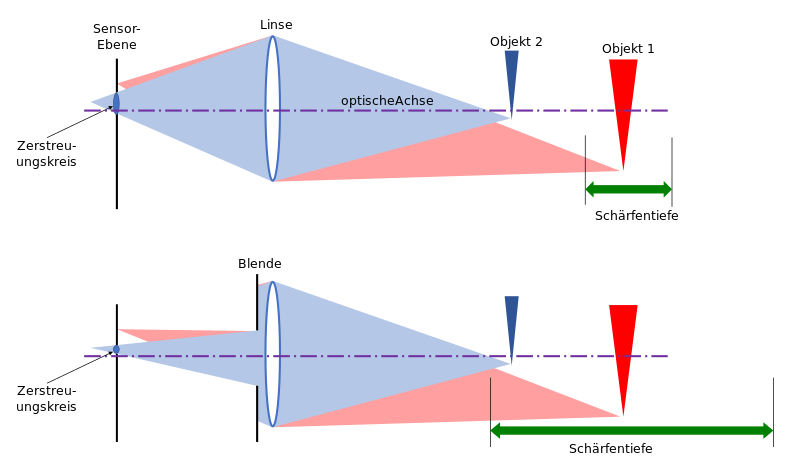
\includegraphics[width=0.7\textwidth]{figures/schaerfentiefe.png}
\end{defi}

\begin{defi}{Zerstreuungskreis}
    % TODO: https://de.wikipedia.org/wiki/Zerstreuungskreis 
    \emph{Zerstreuungskreise} entstehen in der Fotografie bei Unschärfe im Bild, also wenn die Projektion eines Punktes eines Motivs vor beziehungsweise hinter der Projektionsebene liegt oder wenn durch Beugung ein zu projizierender Lichtpunkt unscharf als Beugungsscheibchen abgebildet wird.

    Diese beiden Effekte, die eine Unschärfe hervorrufen, sind bei veränderter Eintrittspupille gegenläufig, so dass sich bei einer bestimmten Blende, der sogenannten kritischen Blende, eine minimale Unschärfe und somit ein maximales Auflösungsvermögen ergibt.

    \centering
    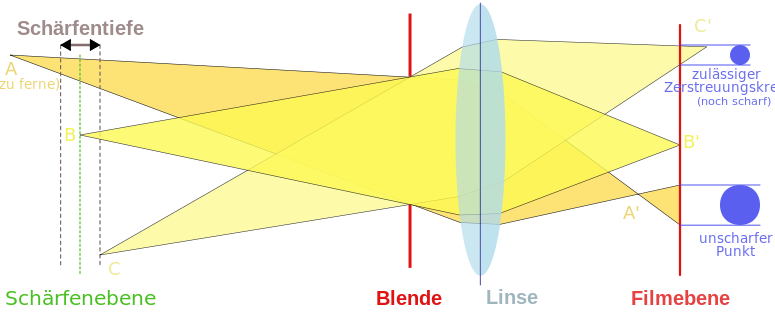
\includegraphics[width=0.6\textwidth]{figures/zerstreuungskreis.png}
\end{defi}

\begin{defi}{Bildkreis}
    % TODO: https://de.wikipedia.org/wiki/Bildkreis 
    Der \emph{Bildkreis} beschreibt in der Fotografie jenen Bereich, den ein Objektiv bildseitig ausleuchten kann. Damit der Film oder der Sensor vollständig beleuchtet wird, muss der Durchmesser des Bildkreises mindestens so groß sein wie die Diagonale des Film- bzw. Sensorformats.

    Der mindestens erforderliche Bildkreisdurchmesser $D$ eines Objektivs errechnet sich als Diagonale des Negativs bzw. rechteckigen Sensors (Breite $B$ und Höhe $H$) nach dem Satz des Pythagoras mit der Formel
    \[
        D = \sqrt{B^2 + H^2}
    \]
\end{defi}

\begin{defi}{Bildwinkel}
    Der \emph{Bildwinkel} definiert den Bereich des Gegenstandsraums, der durch das Objektiv und durch die Ränder des Sensorformats begrenzt wird.

    Außer durch das Bildformat -- Höhe $H$, Breite $B$ bzw. Diagonale $D$ des Bilds -- wird der Bildwinkel $\alpha$ im Wesentlichen nur noch durch die aktuelle Brennweite $f$ des Kameraobjektivs bestimmt.
    Die nachstehende Formel liefert dementsprechend den diagonalen Bildwinkel bei Einstellung des Objektivs auf \enquote{unendlich}:
    \[
        \alpha_d = 2 \cdot \arctan \left( \frac{D}{2 \cdot f} \right)
    \]
    Bei Abbildung näherer Gegenstände dagegen wird die Bildweite $B$ größer als $f$, wodurch sich der Bildwinkel $\alpha$ entsprechend verkleinert.

\end{defi}

\begin{defi}[Kamera]{Sensor}
    % TODO: https://de.wikipedia.org/wiki/Digitalkamera#Bildwandlung 
    Wie bei einer Analogkamera wird das einfallende Licht mit einem Objektiv gesammelt und auf die Filmebene, in Fall einer Digitalkamera auf den \emph{Sensor}, scharfgestellt (fokussiert).

    Der Sensor kann entweder ein Flächensensor oder (selten) ein Zeilensensor sein. Der Flächensensor steht fest in der Filmebene, er registriert gleichzeitig das gesamte Bild. Zeilensensoren werden in Scannerkameras eingesetzt, die nach dem Scannerprinzip funktionieren, das heißt, sie arbeiten ähnlich wie ein Flachbettscanner und tasten das Bild zeilenweise ab: Der Zeilensensor wird mittels Antriebs über die Filmebene gefahren, dabei wird Zeile um Zeile erfasst.

    Die Erfassung der drei Grundfarben kann gleichzeitig im selben Sensor geschehen, der dann für jeden Vollfarb-Pixel drei Subpixel besitzt.
    Die Grundfarben können jedoch auch räumlich getrennt erfasst werden, indem z. B. ein System aus halbdurchlässigen Spiegeln das einfallende Licht auf drei getrennte Sensoren für die drei Grundfarben verteilt.
    Als dritte Möglichkeit können die Grundfarben zeitlich getrennt erfasst werden:
    Gleichzeitig (One-shot-Kameras) oder nacheinander (Three-Shot-Kameras), wobei dann vor jeder Erfassung ein anderer Farbfilter vorgeschaltet wird.
\end{defi}

\begin{defi}[Kamera!Sensor]{Kontrastumfang}
    TODO
\end{defi}

\begin{bonus}[Kamera!Sensor]{Räumliche Diskretisierung}
    TODO
\end{bonus}

\begin{bonus}[Kamera!Sensor]{Funktionsweise}
    TODO
\end{bonus}

\begin{defi}[Kamera!Sensor]{Abtastung}
    TODO
\end{defi}

\begin{defi}[Kamera!Sensor]{Quantisierung}
    TODO
\end{defi} % VL 01
% \section{Bayer-Matrix}

\begin{defi}{Bayer-Matrix}
    % TODO: https://de.wikipedia.org/wiki/Bayer-Sensor 
    Als \emph{Bayer-Sensor} bezeichnet man einen Fotosensor, der -- ähnlich einem Schachbrett -- mit einem Farbfilter überzogen ist, welcher meist zu 50 \% aus Grün und je 25 \% aus Rot und Blau besteht.
    Grün ist in der Flächenzuweisung und somit in der Auflösungsfähigkeit privilegiert, weil der Grün-Anteil in Grautönen beim menschlichen Auge den größten Beitrag zur Helligkeitswahrnehmung und somit auch zur Kontrast-Wahrnehmung und Schärfe-Wahrnehmung leistet:
    72 \% der Helligkeits- und Kontrastwahrnehmung von Grautönen wird durch deren Grünanteil verursacht, dagegen leistet Rot nur 21 \% und Blau nur 7 \%.
    Zudem ist Grün, als die mittlere Farbe im Farbspektrum, diejenige, für die Objektive in der Regel die höchste Schärfe und Auflösung liefern.

    Nach diesem Konzept der \emph{Bayer-Matrix} arbeiten fast alle gebräuchlichen Bildsensoren in digitalen Fotokameras und Filmkameras.

    \centering
    \begin{tabular}{cc}
        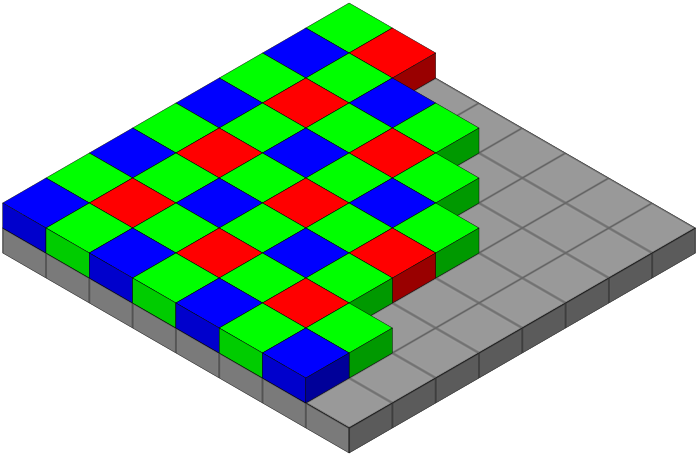
\includegraphics[width=0.5\linewidth]{figures/bayer-matrix.png} &
        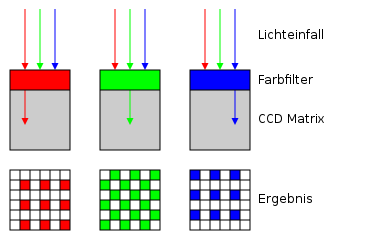
\includegraphics[width=0.5\linewidth]{figures/bayer-sensor.png}
    \end{tabular}
\end{defi}

\begin{defi}{Demosaicing}
    % TODO: https://de.wikipedia.org/wiki/Demosaicing 
    Als \emph{Demosaicing} bezeichnet man in der Digitalfotografie die Rekonstruktion einer farbigen Rastergrafik aus den Helligkeitswerten eines mit Mosaik-Farbfiltern überlagerten Bildsensors.
\end{defi}

\begin{defi}[Demosaicing]{Nearest-Neighbor}
    % TODO: https://ngi-user-guide.readthedocs.io/en/latest/demosaicing/ 
    Die \emph{Nearest-Neighbor-Methode} ist die einfachste Methode zum Demosaicing.
    Jeder interpolierte Pixel wird mit dem nächstgelegenen Pixel der gleichen Farbe gefüllt.

    \centering
    % TODO: https://wiki.apertus.org/index.php/OpenCine.Nearest_Neighbor_and_Bilinear_Interpolation
    \begin{tabular}{cc}
        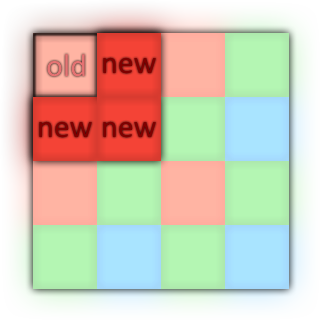
\includegraphics[width=0.15\linewidth]{figures/demosaicing-nearest-neighbour-red-blue.png} &
        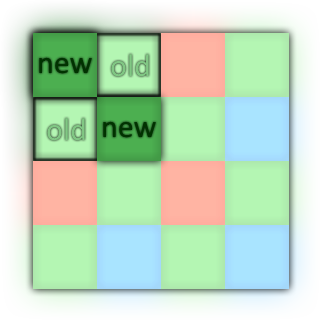
\includegraphics[width=0.15\linewidth]{figures/demosaicing-nearest-neighbour-green.png}
    \end{tabular}
\end{defi}

\begin{defi}[Demosaicing]{Bilineare Interpolation}
    Bei der \emph{Bilinearen Interpolation} werden Farbkomponenten aus den unmittelbaren Nachbarn interpoliert.

    \centering
    % TODO: https://wiki.apertus.org/index.php/OpenCine.Nearest_Neighbor_and_Bilinear_Interpolation
    \begin{tabular}{cccc}
        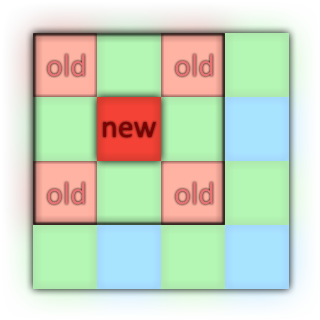
\includegraphics[width=0.15\linewidth]{figures/demosaicing-interpolation-diagonal.png}   &
        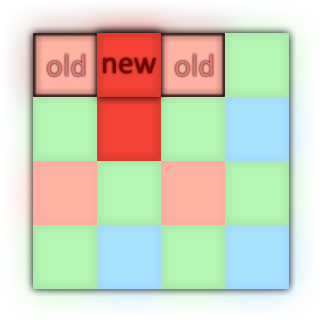
\includegraphics[width=0.15\linewidth]{figures/demosaicing-interpolation-horizontal.png} &
        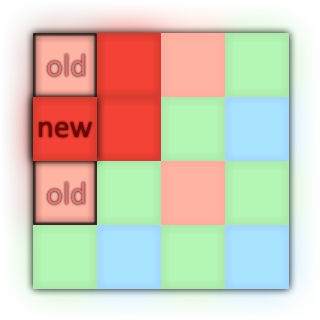
\includegraphics[width=0.15\linewidth]{figures/demosaicing-interpolation-vertical.png}   &
        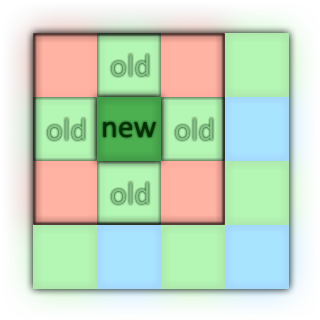
\includegraphics[width=0.15\linewidth]{figures/demosaicing-interpolation-green.png}
    \end{tabular}
\end{defi}

\begin{bonus}[Demosaicing]{Probleme}
    Bei den einfacheren Verfahren des Demosaicing kann es zu Unschärfe und anderen Bildartefakten kommen:
    \begin{itemize}
        \item \enquote{Reißverschlussartige} \emph{Schachbrettmuster} entstehen an Kanten, die nicht entlang der Farbfilter einer Grundfarbe verlaufen;
        \item \emph{Farbverschiebungen} entstehen als Alias-Effekte, wenn die Farbfiltermatrix mit regelmäßig angeordneten Bilddetails interferiert.
    \end{itemize}

    Durch Nachverarbeitung können die Ergebnisse verbessert werden.

    Auch existieren weitere Verfahren, die z. B. kanten- oder frequenzbasiert sind.

    \centering
    % TODO: https://www.semanticscholar.org/paper/Comparison-of-color-demosaicing-methods-Losson-Macaire/37df62621c6a4274e14b0ed7d01a07bc386cd37a/figure/12 
    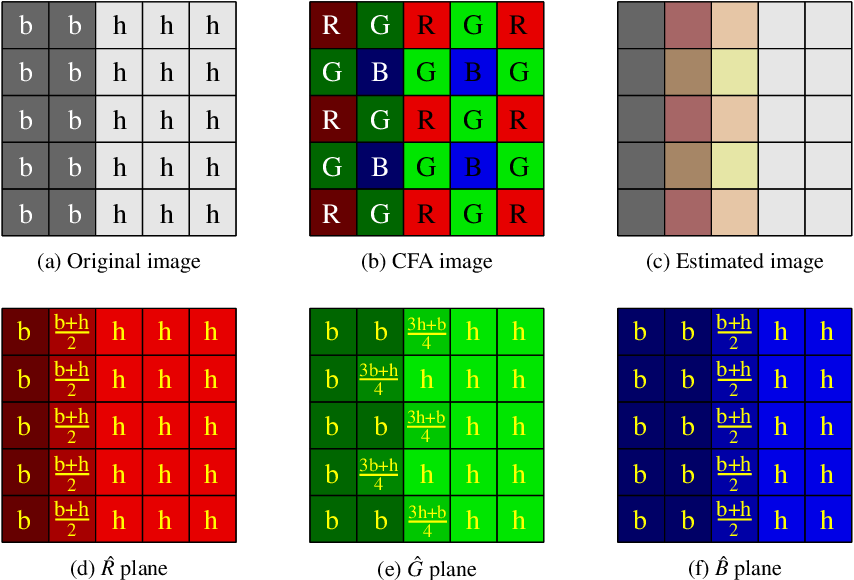
\includegraphics[width=0.75\linewidth]{figures/demosaicing-problems.png}
\end{bonus} % VL 01
% \section{Digitale Bilder}

\begin{defi}{Bild}
    Ein \emph{Bild} ist eine Abbildung $f$ von räumlichen Koordinaten $\mathcal{P}$ auf einen Wertebereich $\mathcal{C}$
    \[
        f: \mathcal{P} \to \mathcal{C}
    \]

    Ein $n$-dimensionales \emph{digitales Bild} mit $m$ Komponenten hat endliche diskrete Bereiche
    \[
        \mathcal{P} \subseteq \mathbb{N}^n, \quad \mathcal{C} \subseteq \mathbb{W}^m, \quad \mathbb{W} \subseteq \{ x \mid 0 \leq x \leq 2^b - 1 \}
    \]

    \begin{tabularx}{\linewidth}{lXl}
        \toprule
        $(n, m, b)$  & Wertebereich                                                                                                                               & Beispiel                 \\
        \midrule
        $(2, 1, 1)$  & $\mathcal{P} \subseteq \mathbb{N}^2, \quad \mathcal{C} \subseteq \mathbb{W}, \quad \mathbb{W} \subseteq \{ x \mid 0 \leq x \leq 1 \}$      & Binärbild                \\
        $(2, 1, 8)$  & $\mathcal{P} \subseteq \mathbb{N}^2, \quad \mathcal{C} \subseteq \mathbb{W}, \quad \mathbb{W} \subseteq \{ x \mid 0 \leq x \leq 255 \}$    & Graustufenbild           \\
        $(3, 1, 16)$ & $\mathcal{P} \subseteq \mathbb{N}^3, \quad \mathcal{C} \subseteq \mathbb{W}, \quad \mathbb{W} \subseteq \{ x \mid 0 \leq x \leq  65535 \}$ & Typisch für CT           \\
        $(2, 3, 8)$  & $\mathcal{P} \subseteq \mathbb{N}^2, \quad \mathcal{C} \subseteq \mathbb{W}^3, \quad \mathbb{W} \subseteq \{ x \mid 0 \leq x \leq 255 \}$  & True Color Fotos         \\
        $(2, 4, 8)$  & $\mathcal{P} \subseteq \mathbb{N}^2, \quad \mathcal{C} \subseteq \mathbb{W}^4, \quad \mathbb{W} \subseteq \{ x \mid 0 \leq x \leq 255 \}$  & Zusätzlicher Alpha-Kanal \\
        \bottomrule
    \end{tabularx}
\end{defi}

\begin{defi}{Tagged Image File Format (TIFF)}
    TODO
\end{defi}

\begin{defi}{Graphics Interchange Format (GIF)}
    TODO
\end{defi}

\begin{defi}{Windows Bitmap (BMP)}
    TODO
\end{defi}

\begin{defi}{Joint Photographic Expert Group (JPEG)}
    TODO
\end{defi}

\begin{defi}{Portable Network Graphics (PNG)}
    TODO
\end{defi}

\begin{defi}{Pixel}
    Die einzelnen Elemente eines 2D-Bildes heißen \emph{Pixel}.
\end{defi}

\begin{defi}{Voxel}
    Die einzelnen Elemente eines 3D-Bildes heißen \emph{Voxel}.
\end{defi}

\begin{defi}{Bildgröße}
    Die \emph{Bildgröße} wird in Pixel (2D) bzw. Voxel (3D) angegeben.
\end{defi}

\begin{defi}{Bildauflösung}
    Die \emph{Bildauflösung} im physikalischen Sinne wird als \emph{Punktdichte} angegeben.

    Die Punktdichte bestimmt die Ausgabegröße in Abhängigkeit der Bildgröße:
    \[
        \si{\ppi} = \frac{\text{Input Size} \ [\si{\pixel}]}{\text{Output Size} \ [\si{\cm}]} \cdot \SI{2,54}{\cm}
    \]
\end{defi}

\begin{defi}[Bild]{Nachbarschaft}
    Oftmals werden in der Bildverarbeitung nur bestimmte Nachbarn eines Pixels betrachtet.

    Die \emph{4-Nachbarschaft} $N_4(p)$ eines Pixels $p$ sind die vertikalen und horizontalen Nachbarn.

    Die \emph{diagonalen Nachbarn} eines Pixels $p$ heißen $N_D(p)$.

    Die \emph{8-Nachbarschaft} $N_8(p)$ eines Pixels $p$ besteht aus $N_4(p)$ und $N_D(p)$.

    TODO: Grafik
\end{defi}


\begin{bonus}[Bild]{Rechenoperationen}
    Digitale Bilder der Höhe $m$ und der Breite $n$ können als Matrizen oder Arrays $M$ interpretiert werden:
    \[
        M_{m.n} =
        \begin{pmatrix}
            m_{0, 0}   & m_{0, 1}   & \cdots & m_{0, n-1}   \\
            m_{1, 0}   & m_{1, 1}   & \cdots & m_{1, n-1}   \\
            \vdots     & \vdots     & \ddots & \vdots       \\
            m_{m-1, 0} & m_{m-1, 1} & \cdots & m_{m-1, n-1}
        \end{pmatrix}
    \]

    Entsprechend können auch elementweise arithmetische Operationen (z. B. Addition, Subtraktion, Multiplikation, Division) durchgeführt werden.

    Konkret beachten muss man, dass \emph{Datentypen} eingehalten werden, durch z. B.
    \begin{itemize}
        \item Konvertierungen in einen passenden Datentypen,
        \item Clipping oder
        \item andere Rechenvorschriften.
    \end{itemize}
\end{bonus}
 % VL 01, VL 02

% Until 06/26/2023
% \section{Bildtransformationen}

\begin{defi}{Affine Transformation}
    % TODO: https://de.wikipedia.org/wiki/Affine_Abbildung
    In der Geometrie und in der Linearen Algebra ist eine \emph{affine Abbildung} (auch \emph{affine Transformation} genannt, insbesondere bei einer bijektiven affinen Abbildung) eine Abbildung zwischen zwei affinen Räumen, bei der \emph{Kollinearität}, \emph{Parallelität} und \emph{Teilverhältnisse} bewahrt bleiben oder gegenstandslos werden.

    Präziser formuliert:
    \begin{enumerate}
        \item Die Bilder von Punkten, die auf einer Geraden liegen (d. h. kollinear sind), liegen wieder auf einer Geraden (\emph{Invarianz der Kollinearität}). Dabei können auch alle -- aber dann alle und nicht nur einige -- Punkte einer Geraden auf einen Punkt abgebildet werden.
        \item Die Bilder zweier paralleler Geraden sind parallel, wenn keine der beiden Geraden auf einen Punkt abgebildet wird.
        \item Drei verschiedene Punkte, die auf einer Geraden liegen (kollineare Punkte), werden so abgebildet, dass das Teilverhältnis ihrer Bildpunkte mit dem der Urbildpunkte übereinstimmt -- es sei denn, alle drei werden auf denselben Bildpunkt abgebildet.
    \end{enumerate}

    Eine bijektive affine Abbildung eines affinen Raumes auf sich selbst wird \emph{Affinität} genannt.
\end{defi}

\begin{bonus}[Affine Transformation]{Taxonomie}

\end{bonus}

\begin{defi}{Homogene Koordinaten}
    Zweidimensionale lineare Transformationen lassen sich einheitlich durch eine $3 \times 3$-Matrix darstellen.

    Die Transformation eines Punktes $(x, y)$ zu einem neuen Punkt $(x', y')$ durch eine beliebige Folge von Translationen, Rotationen und Skalierungen wird beschrieben durch:
    \[
        \begin{pmatrix}
            a & b & c \\
            d & e & f \\
            0 & 0 & 1
        \end{pmatrix}
        \begin{pmatrix}
            x \\ y \\ 1
        \end{pmatrix}
        =
        \begin{pmatrix}
            x' \\ y' \\ 1
        \end{pmatrix}
    \]

    Dabei beschreibt die Teilmatrix aus den Komponenten $a$, $b$, $d$ und $e$ Rotation und Skalierung und die Teilmatrix bestehend aus $c$ und $f$ eine Translation.

    Zwei oder mehrere affine Transformationen, die hintereinander ausgeführt werden sollen, lassen sich Verketten (\emph{Konkatenation}) und durch die Anwendung einer Transformationsmatrix ausführen.

    Homogene Koordinaten sind invariant gegenüber Skalierung.
\end{defi}

\begin{defi}[Affine Transformation]{Translation}
    % TODO: https://www.gm.th-koeln.de/~konen/WPF-BV/BV08.pdf 
    Die Position $p'$ eines Pixels $p$ nach einer Verschiebung (\emph{Translation}) um $t_x$ in positive $x$-Richtung und $t_y$ in positive $y$-Richtung wird wie folgt berechnet:
    \[
        p' = p + t =
        \begin{pmatrix}
            x + t_x \\
            y + t_y
        \end{pmatrix}
    \]

    Die Transformationsgleichung für die Translation sieht wie folgt aus:
    \[
        \begin{pmatrix}
            1 & 0 & t_x \\
            0 & 1 & t_y \\
            0 & 0 & 1
        \end{pmatrix}
        \begin{pmatrix}
            x \\ y \\ 1
        \end{pmatrix}
        =
        \begin{pmatrix}
            x' \\ y' \\ 1
        \end{pmatrix}
    \]

    Die Translation ist eine affine Abbildung.

    TODO: Grafik
\end{defi}

\begin{defi}[Affine Transformation]{Rotation}
    % TODO: https://www.gm.th-koeln.de/~konen/WPF-BV/BV08.pdf 
    Die Position $p'$ eines Pixels $p$ nach einer Drehung (\emph{Rotation}) um den Ursprung $(0, 0)$ mit dem Winkel $\alpha$ wird wie folgt berechnet:
    \[
        p' =
        \begin{pmatrix}
            \cos \alpha & -\sin \alpha \\
            \sin \alpha & \cos \alpha
        \end{pmatrix}
        \begin{pmatrix}
            x \\
            y
        \end{pmatrix}
    \]

    Die Transformationsgleichung für die Rotation sieht wie folgt aus:
    \[
        \begin{pmatrix}
            \cos \alpha  & \sin \alpha & 0 \\
            -\sin \alpha & \cos \alpha & 0 \\
            0            & 0           & 1
        \end{pmatrix}
        \begin{pmatrix}
            x \\ y \\ 1
        \end{pmatrix}
        =
        \begin{pmatrix}
            x' \\ y' \\ 1
        \end{pmatrix}
    \]

    Die Rotation ist eine affine Abbildung.

    TODO: Grafik
\end{defi}

\begin{defi}[Affine Transformation]{Skalierung}
    % TODO: https://www.gm.th-koeln.de/~konen/WPF-BV/BV08.pdf 
    Die Position $p'$ eines Pixels $p$ nach einer \emph{Skalierung} relativ zum Ursprung $(0, 0)$, mit dem horizontalen Skalierungsfaktor $s_x$ und dem vertikalen Skalierungsfaktor $s_y$ wird wie folgt berechnet:
    \[
        p' = p \circ s =
        \begin{pmatrix}
            x \cdot s_x \\
            y \cdot s_y
        \end{pmatrix}
    \]

    Die Transformationsgleichung für die Skalierung sieht wie folgt aus:
    \[
        \begin{pmatrix}
            s_x & 0   & 0 \\
            0   & s_y & 0 \\
            0   & 0   & 1
        \end{pmatrix}
        \begin{pmatrix}
            x \\ y \\ 1
        \end{pmatrix}
        =
        \begin{pmatrix}
            x' \\ y' \\ 1
        \end{pmatrix}
    \]

    Die Skalierung ist eine affine Abbildung.

    TODO: Grafik
\end{defi}

\begin{defi}[Affine Transformation]{Scherung}
    % TODO: https://www.gm.th-koeln.de/~konen/WPF-BV/BV08.pdf 
    Die Position $p'$ eines Pixels $p$ nach einer \emph{Scherung} (Transvektion) TODO
    \[
        p' =
        \begin{pmatrix}
            1   & c_x \\
            c_y & 1
        \end{pmatrix}
        \begin{pmatrix}
            x \\
            y
        \end{pmatrix}
    \]

    Die Transformationsgleichung für die Scherung sieht wie folgt aus:
    \[
        \begin{pmatrix}
            1   & c_x & 0 \\
            c_y & 1   & 0 \\
            0   & 0   & 1
        \end{pmatrix}
        \begin{pmatrix}
            x \\ y \\ 1
        \end{pmatrix}
        =
        \begin{pmatrix}
            x' \\ y' \\ 1
        \end{pmatrix}
    \]

    Die Scherung ist eine affine Abbildung.

    TODO: Grafik
\end{defi}

\begin{defi}[TODO]{Forward Mapping}
    TODO

    TODO: Grafik
\end{defi}

\begin{defi}[TODO]{Backward Mapping}
    TODO

    TODO: Grafik
\end{defi}

\begin{defi}[TODO]{Interpolation}
    TODO

    TODO: Grafik
\end{defi}

\begin{defi}{Projektive Transformation}
    \emph{Projektive Abbildungen} sind Abbildungen, welche Geraden in Geraden überführen.

    \begin{itemize}
        \item Lösung als Lineares Gleichungssystem
              \begin{itemize}
                  \item 4 Punktepaare
                  \item Ein Element (unten rechts) wird auf einen festen Wert gesetzt (meist auf 1)
                  \item Lösung des Gleichungssystems nutzt Pseudoinverse
              \end{itemize}
        \item Lösung mit Singulärwertzerlegung (SVD)
              \begin{itemize}
                  \item Optimierungsproblem mit N Punktepaare
                  \item Algebraische Distanz wird minimiert
                  \item SVD wird zur Lösung verwendet
              \end{itemize}
        \item Nicht-lineare Lösung
              \begin{itemize}
                  \item Optimierungsproblem mit N Punktepaaren
                  \item Euklidische Distanzen zw. Punktepaaren werden minimiert
                  \item Lösung wird iterativ gesucht
              \end{itemize}
    \end{itemize}

    TODO: Grafik, Formulierung
\end{defi} % VL 02
% \section{Histogramme}

\begin{defi}{Histogramm}
    % TODO: https://de.wikipedia.org/wiki/Histogramm#Histogramm_in_der_Bildverarbeitung 
    In der digitalen Bildverarbeitung versteht man unter einem \emph{Histogramm} die statistische Häufigkeit der Grauwerte bzw. der Farbwerte in einem Bild.

    Das Histogramm eines Bildes erlaubt eine Aussage über die vorkommenden Grau- bzw. Farbwerte und über Kontrastumfang und Helligkeit des Bildes.

    In einem farbigen Bild kann entweder ein Histogramm über alle möglichen Farben oder Histogramme über die einzelnen Farbkanäle erstellt werden.
    Letzteres ist meist sinnvoller, da die meisten Verfahren auf Grauwertbildern basieren und so die sofortige Weiterverarbeitung möglich ist.

    Die Anzahl der Farbkanäle in einem Bild ist abhängig vom Modus, das heißt pro Farbauszug gibt es einen Kanal.
    Daher haben CMYK-Bilder vier Farbkanäle, RGB-Farbbilder nur drei.
\end{defi}

\begin{defi}{Grauwert-Histogramm}
    Ein \emph{Grauwert-Histogramm} ist eine visuelle Darstellung der Häufigkeitsverteilung der Intensitätswerte.


\end{defi}

\begin{defi}[Histogramm!Interpretation]{Belichtung}

\end{defi}

\begin{defi}[Histogramm!Interpretation]{Kontrast}

\end{defi}

\begin{defi}[Histogramm!Interpretation]{Kontrastumfang}

\end{defi}

\begin{defi}[Histogramm]{Mittelwert}

\end{defi}

\begin{example}[Histogramm]{Mittelwert}

\end{example}

\begin{defi}[Histogramm]{Standardabweichung}

\end{defi}

\begin{example}[Histogramm]{Standardabweichung}

\end{example}

\begin{defi}{Farb-Histogramm}

\end{defi}

\begin{defi}{Kumulatives Histogramm}

\end{defi}

 % VL 02

% Until 06/27/2023
% \section{Punktoperatoren}

\begin{defi}{Punktoperator}
    Als \emph{Punktoperatoren} bezeichnet man eine umfangreiche Klasse von Bildverarbeitungsoperationen in der digitalen Bildverarbeitung, die sich -- gegenüber lokalen und globalen Operatoren -- dadurch auszeichnen, dass bei allen Verfahren dieser Klasse ein neuer Farb- oder Grauwert eines Pixels allein in Abhängigkeit von seinem eigenen bisherigen Farb- oder Grauwert und seiner eigenen bisherigen Position im Bild berechnet wird, ohne sich dabei um seine Nachbarschaft und/oder den Kontext des Pixels zu kümmern.

    Ein Punktoperator $T$ ordnet einem Eingabebild $f$ durch Transformation der Grauwerte der einzelnen Pixel ein Ergebnisbild $f^*$ zu.
    Der Grauwert $f(x,y)$ eines Pixels $(x,y)$ wird dabei nur in Abhängigkeit vom Grauwert selbst und eventuell von der Position des Pixels im Bild modifiziert:
    \[
        f^*(x, y) = T_{xy}(f(x, y))
    \]

    Ist die Transformation von der Position des Pixels im Bild abhängig, so heißt sie \emph{inhomogen}.
    Die Indizes $x$ und $y$ von $T$ sollen diese Abhängigkeit verdeutlichen.

    In der Mehrheit der Fälle kommen jedoch \emph{homogene} Transformationen zum Einsatz, bei denen diese Abhängigkeit nicht gegeben ist.
    Die Indizes werden dann überflüssig:
    \[
        f^*(x, y) = T(f(x, y))
    \]
\end{defi}

\begin{defi}[Homogener Punktoperator]{Helligkeit}
    Um die \emph{Helligkeit} zu verändern, wird zu jedem Pixel ein konstanter Wert $c$ addiert:
    \[
        T_{\text{Brightness}}(f) = f + c
    \]

    TODO: Beispiel

    Eine Änderung der Helligkeit führt zu einer \emph{Histogrammverschiebung}.

    TODO: Beispiel
\end{defi}

\begin{defi}[Homogener Punktoperator]{Kontrast}
    Um den \emph{Kontrast} zu verändern, wird jeder Pixel mit einem konstanten Wert $c$ multipliziert:
    \[
        T_{\text{Contrast}}(f) = f \cdot c
    \]

    TODO: Beispiel

    Eine Änderung des Kontrasts führt zu einer \emph{Histogrammspreizung}.

    TODO: Beispiel
\end{defi}

\begin{defi}[Homogener Punktoperator!Kontrast]{Automatischer Kontrast}
    Die \emph{automatische Kontrastanpassung} soll Pixelwerte so verändern, dass der verfügbare Wertebereich ausgenutzt wird.

    Unter den Annahmen, dass
    \begin{itemize}
        \item der Wertebereich durch $[v_{\min}; v_{\max}]$ beschränkt ist, und
        \item $v_{\low}$ und $v_{\high}$ der kleinste bzw. größte vorhandene Pixelwert sind,
    \end{itemize}
    gilt:
    \[
        T_{\text{Auto-Contrast}}(f) = v_{\min} + (f - v_{\low}) \cdot \frac{v_{\max} - v_{\min}}{v_{\high} - v_{\low}}
    \]

    Diese Variante des automatischen Kontrasts ist stark beeinflussbar durch wenige Pixel, die nicht repräsentativ sind (\enquote{Ausreißer}).

    TODO: Beispiel

    TODO: Beispiel
\end{defi}

\begin{defi}[Homogener Punktoperator!Kontrast]{Verbesserter automatischer Kontrast}
    Die \emph{verbesserte automatische Kontrastanpassung} bestimmt einen Prozentsatz $s_{\low}$ bzw. $s_{\high}$, der Pixel am oberen und unteren Ende in die Sättigung treiben soll.

    Analog zu diesen Perzentilen müssen zwei Schwellwerte $v'_{\low}$ und $v'_{\high}$ gefunden werden:
    \[
        v'_{\low} = \min \{ i \mid H(i) \geq \width \cdot \height \cdot s_{\low} \}
    \]
    \[
        v'_{\high} = \min \{ i \mid H(i) \geq \width \cdot \height \cdot (1 - s_{\high}) \}
    \]
    Werte außerhalb von $v'_{\low}$ und $v'_{\high}$ werden dann auf $v_{\min}$ bzw. $v_{\high}$ abgebildet, Werte dazwischen linear auf das Intervall $[v_{\min}; v_{\max}]$:
    \[
        T_{\text{Improved-Auto-Contrast}}(f) =
        \begin{cases}
            v_{\min}                                                                            & f \leq v'_{\low}           \\
            v_{\min} + (f - v'_{\low}) \cdot \frac{v_{\max} - v_{\min}}{v'_{\high} - v'_{\low}} & v'_{\low} < f < v'_{\high} \\
            v_{\max}                                                                            & f \geq v'_{\high}
        \end{cases}
    \]

    TODO: Beispiel

    TODO: Beispiel
\end{defi}

\begin{defi}[Homogener Punktoperator]{Invertierung}
    Bei der \emph{Invertierung} werden alle Pixel negiert und zum maximalen Wert $c_{\max}$ des Wertebereichs addiert:
    \[
        T_{\text{Invert}}(f) = -f + c_{\max} = c_{\max} - f
    \]

    TODO: Beispiel

    TODO: Beispiel
\end{defi}

\begin{defi}[Homogener Punktoperator]{Thresholding}
    \emph{Schwellwertverfahren} (\emph{Thresholding}) teilen die Pixelwerte abhängig von einem Schwellwert $c$ in zwei Klassen ein
    \[
        T_{\text{Threshold}}(f) =
        \begin{cases}
            v_a & f > c    \\
            v_b & f \leq c
        \end{cases}
    \]

    TODO: Beispiel

    TODO: Beispiel
\end{defi}

\begin{defi}[Homogener Punktoperator]{Transferfunktion}
    TODO

    TODO: Beispiel

    TODO: Beispiel
\end{defi}

\begin{defi}[Homogener Punktoperator]{Windowing}
    TODO

    TODO: Beispiel

    TODO: Beispiel
\end{defi}

\begin{defi}[Homogener Punktoperator]{Histogrammausgleich}
    Das Ziel des \emph{Histogrammausgleichs} ist, eine Punktoperation zu finden und anzuwenden, so dass die Histogramme der veränderten Bilder eine Gleichverteilung approximieren.

    Nur approximieren daher, dass globale Punktoperatoren Histogrammeinträge nur verschieben und mit anderen Einträgen verschmelzen, aber niemals trennen können.
    Dadurch können z. B. individuelle Peaks im Histogramm nicht beseitigt werden.

    Ein Histogrammausgleich kann die Farbzusammensetzung durcheinander bringen.
    Bilder wirken dadurch unnatürlich.

    Ein Histogrammausgleich eignet sich am besten für Grauwertbilder, oder in einem anderen Farbraum (dort nur auf dem Luminanzkanal).

    TODO: Beispiel

    TODO: Beispiel
\end{defi}

\begin{example}[Homogener Punktoperator!Histogrammausgleich]{Gleichverteilung}
    Bei einem \emph{gleichverteilten} Histogramm ist das kumulative Histogramm ungefähr linear.

    Das Problem des Histogrammausgleichs lässt sich also so umformulieren, dass stattdessen ein Punktoperator gefunden werden soll, der das kumulative Histogramm ungefähr linear werden lässt.

    Die Einträge können im kumulativen Histogramm wie folgt nach rechts oder links verschoben werden:
    \[
        T_{\text{Equalize}}(f) = \left\lfloor H(f) \cdot \frac{K - 1}{\width \cdot \height} \right\rfloor
    \]

    TODO: Beispiel

    TODO: Beispiel
\end{example}

\begin{defi}[Inhomogener Punktoperator]{Gammakorrektur}
    TODO

    TODO: Beispiel

    TODO: Beispiel
\end{defi} % VL 03
% \section{Filter}

\begin{defi}{Filter}
    % TODO: https://de.wikipedia.org/wiki/Bildverarbeitung#Operationen_der_Bildverarbeitung 
    \emph{Nachbarschaftsoperationen} (\emph{Filter}) verwenden sowohl einen Punkt als auch eine bestimmte Menge seiner Nachbarn als Eingabe, errechnen aus ihnen ein Ergebnis und schreiben dieses an die Koordinate des Referenzpunktes in das Zielbild.

    Eine sehr verbreitete Art von Nachbarschaftsoperationen sind die Faltungsfilter (\emph{Convolutional Filter}).
    Hierbei werden die Helligkeit- oder Farbwerte gemäß einem Filterkern miteinander verrechnet um das Ergebnis zu bilden.

    Bei Filtern wird ein Pixel für die Berechnung von mehr als einem neuen Pixel benötigt -- im Kontrast zu Punktfiltern.
    Daher benötigt es einer Kopie.

    Filterkerne haben üblicherweise eine ungerade Anzahl an $(2k + 1)$ Spalten und $(2l + 1)$ Reihen ($k, l \in \mathbb{N} \setminus \{0\}$).
    Für ein Bild der Größe $m \times n$ kann ein Filter für die Bildkoordinaten $(x, y)$ berechnet werden, wenn
    \begin{itemize}
        \item $k \leq x \leq m - k - 1$ und
        \item $l \leq y \leq n - l - 1$
    \end{itemize}

    TODO: Linear vs. nicht-linear
\end{defi}

\begin{defi}[Filter]{Glättung}
    Bei einem \emph{Glättungsfilter} werden lokale Intensitäten \enquote{geglättet}.

    TODO
\end{defi}

\begin{defi}[Filter]{Ableitung}
    Bei \emph{Differenzfiltern} (\emph{Ableitung}) sind einige Koeffizienten negativ.

    Das Ergebnis kann interpretiert werden als Summe von allen Pixeln mit korrespondierenden positiven Koeffizienten minus Summe von allen Pixeln mir korrespondierenden negativen Koeffizienten -- analog zur Berechnung von Ableitungen.

    Da Bilder keine kontinuierlichen Funktionen sind, werden Ableitung mit Finiten Differenzen berechnet.

    TODO
\end{defi}

\begin{example}[Filter!Ableitung]{Laplace-Operator}
    Der einfachste isotropische 2. Ableitungsoperator ist der \emph{Laplace-Operator}:
    \[
        \nabla^2 f = \frac{\partial^2 f}{\partial x^2} + \frac{\partial^2 f}{\partial y^2}
    \]

    Nach Diskretisierung mit finiten Differenzen erhält man:
    \begin{alignat*}{2}
        \frac{\partial^2 f}{\partial x^2} & = f(x + 1, y) + f(x - 1, y) - 2 f(x, y)                           \\
        \frac{\partial^2 f}{\partial y^2} & = f(x, y + 1) + f(x, y - 1) - 2 f(x, y)                           \\
        \nabla^2 f                        & = f(x + 1, y) + f(x - 1, y) f(x, y + 1) + f(x, y - 1) - 4 f(x, y)
    \end{alignat*}

    TODO
\end{example}

\begin{defi}[Filter]{Glättung}
    Bei einem \emph{Glättungsfilter} werden lokale Intensitäten \enquote{geglättet}.

    TODO
\end{defi}

\begin{defi}[Filter]{Unscharfmaskierung}
    % TODO: https://de.wikipedia.org/wiki/Unscharfmaskierung 
    \emph{Unscharfmaskierung} (\enquote{Selektive Schärfe}) bezeichnet eine Filtermethode, bei der der Schärfeeindruck eines Fotos mit Hilfe einer unscharfen Kopie dieses Fotos erhöht wird.

    TODO
\end{defi}

\begin{defi}{Separierbarkeit}
    \emph{Separierbarkeit} bezeichnet die Möglichkeit einen 2D Filterkern in zwei 1D Filterkerne zu trennen.

    Ein 2D Filterkern ist separierbar, wenn er als dyadisches Produkt ausgedrückt werden kann:

    TODO
\end{defi}

\begin{defi}{Randbehandlung}
    Ohne spezielle \emph{Randbehandlung} würde jeder Filter die Größe des Bildes reduzieren.

    Es existieren verschiedene Methoden:
    \begin{itemize}
        \item Pixel am Rand, die nicht verarbeitet wurden, auf einen konstanten Wert setzen (z. B. schwarz).
              \begin{itemize}
                  \item einfache Methode
                  \item Bildgröße wird reduziert
              \end{itemize}
        \item Pixel am Rand, die nicht verarbeitet wurden, auf den Originalwert des Bildes setzen.
              \begin{itemize}
                  \item einfache Methode
                  \item sichtbarer Unterschied
              \end{itemize}
        \item Bild um zusätzliche Pixel erweitern, dann normal filtern und anschließend beschneiden.
              \subitem Erweitern mit:
              \begin{itemize}
                  \item konstantem Wert
                        \begin{itemize}
                            \item sichtbare Artefakte
                        \end{itemize}
                  \item kopierten Randpixeln
                        \begin{itemize}
                            \item geringe Artefakte
                            \item oft genutzt
                        \end{itemize}
                  \item gespiegeltem Bild
                        \begin{itemize}
                            \item nur bei großen Kernen Vorteile
                        \end{itemize}
                  \item periodischer Fortsetzung des Bildes
                        \begin{itemize}
                            \item sichtbare Artefakte
                            \item theoretische Vorteile bzgl. Spektralanalyse
                        \end{itemize}
              \end{itemize}
    \end{itemize}

    TODO
\end{defi}

\begin{defi}[Nicht-linearer Filter]{Minimum- und Maximum-Filter}
    \emph{Minimum-} und \emph{Maximum-Filter} ersetzen den aktuellen Pixel mit dem Minimum bzw. Maximum in der Filterregion.

    TODO: Salt and Pepper Noise
\end{defi}

\begin{defi}[Nicht-linearer Filter]{Median-Filter}
    Ein \emph{Median-Filter} ersetzt den aktuellen Pixel mit dem Median der Filterregion.

    Median-Filter eignen sich gut, um Salt- and Pepper-Rauschen zu entfernen, sind aber weniger gut bei Gaußschem Rauschen.
    Außerdem glätten sie das Bild im Vergleich zu linearen Filtern viel weniger und erhalten Kanten.

    TODO: Salt and Pepper Noise
\end{defi} % VL 04

% Until 06/28/2023
\section{Kanten und Konturen}

\begin{defi}{Kante}
    \emph{Kanten} (lokale Intensitätsänderungen) spielen eine wichtige Rolle bei der Wahrnehmung und Interpretation.
    Der Schärfeeindruck eines Bildes korreliert mit Kantenstruktur.

    Kanten sind überall dort wo sich im Bild die lokale Intensität stark verändert:
    \[
        f'(x) = \frac{\partial f(x)}{\partial x} \gg 0
    \]

    In 2D sind die partiellen Ableitungen eines Bildes $I$ in $x$- bzw. $y$-Richtung gegeben durch:
    \[
        I_x = \frac{\partial}{\partial x} I(x, y), \quad I_y = \frac{\partial}{\partial y} I(x, y)
    \]
    Der Gradient an der Stelle $(x, y)$ ist der Vektor
    \[
        \nabla I(x, y) = \begin{bmatrix}
            I_x \\
            I_y
        \end{bmatrix}
    \]

    TODO: Grafik
\end{defi}

\begin{example}[Kante]{Sprungkante}
    % TODO: https://www.researchgate.net/figure/Type-of-Edges-a-Step-Edge-b-Ramp-Edge-c-Line-Edge-d-Roof-Edge_fig1_228349759 
    Eine \emph{Sprungkante} (\emph{Step Edge}) tritt auf, wenn die Pixelwerte abrupt ansteigen oder abfallen.

    TODO: Grafik
\end{example}

\begin{example}[Kante]{Rampenkante}
    % TODO: https://www.researchgate.net/figure/Type-of-Edges-a-Step-Edge-b-Ramp-Edge-c-Line-Edge-d-Roof-Edge_fig1_228349759 
    Eine \emph{Rampenkante} (\emph{Ramp Edge}) tritt auf, wenn die Pixelwerte langsam ansteigen oder abfallen.

    TODO: Grafik
\end{example}

\begin{example}[Kante]{Linienkante}
    % TODO: https://www.researchgate.net/figure/Type-of-Edges-a-Step-Edge-b-Ramp-Edge-c-Line-Edge-d-Roof-Edge_fig1_228349759 
    Eine \emph{Linienkante} (\emph{Line Edge}) tritt auf, wenn die Pixelwerte abrupt ansteigen und dann abfallen.

    TODO: Grafik
\end{example}

\begin{example}[Kante]{Dachkante}
    % TODO: https://www.researchgate.net/figure/Type-of-Edges-a-Step-Edge-b-Ramp-Edge-c-Line-Edge-d-Roof-Edge_fig1_228349759 
    Eine \emph{Dachkante} (\emph{Roof Edge}) tritt auf, wenn die Pixelwerte langsam ansteigen und dann abfallen.

    TODO: Grafik
\end{example}

\begin{defi}{Kantennormale}
    Die \emph{Kantennormale} ist der Einheitsvektor $\frac{\nabla I}{| \nabla I |}$, der in Richtung der größten Intensitätsänderung zeigt.
\end{defi}

\begin{defi}{Kantenrichtung}
    Die \emph{Kantenrichtung} $\theta(x, y)$ (\emph{Gradient Direction}) ist der Einheitsvektor entlang der Kante:
    \[
        \tan (\theta(x, y)) = \frac{I_y(x, y)}{I_x(x, y)} \quad \implies \quad \theta(x, y) = \arctan \left( \frac{I_y(x, y)}{I_x(x, y)} \right)
    \]

    Sie ist orthogonal zur Kantennormalen.
\end{defi}

\begin{defi}{Kantenposition}
    Die \emph{Kantenposition} ist die Position $(x, y)$ im konkreten Bild $I$ der Kante.
\end{defi}

\begin{defi}{Kantenstärke}
    Die \emph{Kantenstärke} $| \nabla I |$ (\emph{Gradient Magnitude}) ist der lokale Bildkontrast entlang der Kantennormalen:
    \[
        | \nabla I | = \sqrt{I_x^2 + I_y^2} \quad \text{(alternativ Betrag oder Maximum)}
    \]

    Sie ist invariant gegenüber Rotation und die Basis für viele Kantendetektoren.
\end{defi}

\begin{defi}{Kantendetektor}
    % TODO: https://de.wikipedia.org/wiki/Kantendetektion 
    Ein \emph{Kantendetektor} berechnet in der Regel den Farbwertgradienten an jedem einzelnen Pixel eines Bildes durch Untersuchung eines den Punkt umgebenden Bereiches.

    Dieser Vorgang erfolgt durch diskrete Faltung des Bildes mit einer Faltungsmatrix, dem Kantenoperator.
    Dieser definiert dabei die Größe des zu untersuchenden Umfeldes und mit welcher Gewichtung dessen einzelne Pixel in die Berechnung eingehen.

    Der Kantenoperator ermittelt für das zentrale Pixel aus der Umgebung quasi einen mittleren Wert für den Gradienten.
    Führt man diese Operation für alle Pixel im Bild durch, so kann man aus der resultierenden Matrix der Gradienten ein neues Bild zusammensetzen, das Kantenbild genannt wird.
    Auf ihm heben sich die Kanten zwischen homogenen Bereichen ab, da an diesen Stellen ein vergleichsweise großer Gradient der Farbwerte vorliegt.

    Wendet man den Kantenoperator auf das Ergebnisbild an, so kann man quasi die zweite Ableitung bilden, d. h., es werden die Änderungen des Helligkeits-Gradienten sichtbar.
    Die Kanten treten in der zweiten Ableitung meist am deutlichsten hervor.

    Feine Kanten können hierbei jedoch untergehen und bleiben unentdeckt.

    Der größte Unterschied verschiedener Kantendetektoren besteht im Allgemeinen im verwendeten Kantenoperator.

    Für eine korrekte \emph{Kantendetektion} sind in der Regel vier Schritte notwendig:
    \begin{enumerate}
        \item \emph{Glätten}: Unterdrücke so viel Rauschen wie möglich, ohne die echten Kanten zu zerstören.
        \item \emph{Verbesserung}: Wende einen Filter an, um die Qualität der Bildränder zu verbessern.
        \item \emph{Erkennung}: Bestimme, welche Pixel als Rauschen verworfen werden sollen und welche beibehalten werden sollte. Normalerweise liefert die Schwellenwertbildung das Kriterium, das für die Erkennung verwendet wird.
        \item \emph{Lokalisierung}: Bestimme die genaue Position einer Kante. Für einige Anwendungen kann es erforderlich sein, die Position einer Kante genauer als den Abstand zwischen den Pixeln zu bestimmen. Kantenverdünnung und Verknüpfung sind in der Regel in diesem Schritt erforderlich.
    \end{enumerate}
\end{defi}

\begin{defi}[Kantendetektor]{Prewitt-Operator}
    % TODO: https://de.wikipedia.org/wiki/Prewitt-Operator
    Der \emph{Prewitt-Operator} berechnet zwei Gradientenbilder $G_x$ und $G_y$ in horizontaler und vertikaler Richtung eines Grauwertbildes $I$:
    \[
        G_x = \begin{bmatrix}
            1 & 0 & -1 \\
            1 & 0 & -1 \\
            1 & 0 & -1
        \end{bmatrix}
        \ast I
        , \quad
        G_y = \begin{bmatrix}
            1  & 1  & 1  \\
            0  & 0  & 0  \\
            -1 & -1 & -1
        \end{bmatrix}
        \ast I
    \]

    Die Kantenstärke $G$ und die Kantenrichtung $\theta$ werden wie folgt berechnet:
    \[
        G = \sqrt{G_x^2 + G_y^2}, \quad \theta = \arctan \left( \frac{G_y}{G_x} \right)
    \]

    Durch Ausnutzung der Separierbarkeit kann die Rechenzeit reduziert werden.

    TODO: Grafik / Beispiel
\end{defi}

\begin{defi}[Kantendetektor]{Sobel-Operator}
    % https://de.wikipedia.org/wiki/Sobel-Operator
    Der \emph{Sobel-Operator} berechnet zwei Gradientenbilder $G_x$ und $G_y$, die für ein Bild $I$ jeweils die erste Ableitung der Bildpunkt-Helligkeitswerte bestimmen, wobei gleichzeitig orthogonal zur Ableitungsrichtung geglättet wird:
    \[
        G_x =
        \underbrace{
            \begin{bmatrix}
                1 \\
                2 \\
                1
            \end{bmatrix}
            \ast
            \begin{bmatrix}
                +1 & 0 & -1
            \end{bmatrix}
        }_{S_x}
        \ast I =
        \underbrace{
            \begin{bmatrix}
                1 & 0 & -1 \\
                2 & 0 & -2 \\
                1 & 0 & -1
            \end{bmatrix}
        }_{S_x}
        \ast I
    \]
    \[
        G_y =
        \underbrace{
            \begin{bmatrix}
                +1 \\
                0  \\
                -1
            \end{bmatrix}
            \ast
            \begin{bmatrix}
                1 & 2 & 1
            \end{bmatrix}
        }_{S_y}
        \ast I =
        \underbrace{
            \begin{bmatrix}
                1  & 2  & 1  \\
                0  & 0  & 0  \\
                -1 & -2 & -1
            \end{bmatrix}
        }_{S_y}
        \ast I
    \]
    Dabei wird die $x$-Koordinate als nach rechts und die $y$-Koordinate als nach unten wachsend angesehen.

    Die Kantenstärke $G$ und die Kantenrichtung $\theta$ werden wie folgt berechnet:
    \[
        G = \sqrt{G_x^2 + G_y^2}, \quad \theta = \arctan \left( \frac{G_y}{G_x} \right)
    \]


    Durch Ausnutzung der Separierbarkeit kann die Rechenzeit deutlich reduziert werden.

    TODO: Grafik / Beispiel
\end{defi}

\begin{defi}[Kantendetektor]{Marr-Hildreth-Operator}
    % TODO: https://de.wikipedia.org/wiki/Marr-Hildreth-Operator
    Der \emph{Marr-Hildreth-Operator} oder \emph{Laplacian of Gaussian} (\emph{LoG}) ist eine spezielle Form eines diskreten Laplace-Filters.

    Der Filterkernel wird durch die Anwendung des Laplace-Operators auf eine Gauß-Funktion erstellt.

    Da seine Form der eines mexikanischen Sombreros ähnelt, ist er auch als Mexican Hat oder Sombrerofilter bekannt.

    Ausgangspunkt für die Erzeugung des Filterkernels ist die Gauß-Funktion in 2D:
    \[
        f(x,y) = \frac {1}{2\pi \sigma^{2}} e^{-\frac {x^{2}+y^{2}}{2\sigma ^{2}}}
    \]

    Wendet man den Laplace-Operator auf die Gauß-Funktion an, erhält man die kontinuierliche Repräsentation des LoG:
    \[
        g(x,y) = \frac {\partial ^{2}f(x,y)}{\partial x^{2}} + \frac {\partial^{2}f(x,y)}{\partial y^{2}}
    \]
    \[
        g(x,y) = -\frac {1}{\pi \sigma ^{4}} e^{-\frac {x^{2}+y^{2}}{2\sigma ^{2}}} \left(1-{\frac {x^{2}+y^{2}}{2\sigma ^{2}}}\right)
    \]

    Um diese Funktion in der Bildverarbeitung zu nutzen, wird der kontinuierliche LoG diskret approximiert für Kernel ungerader Kantenlänge $k \in 2 \mathbb{N} + 1$.

    Der LoG findet im Grunde genommen keine Kanten, sondern Gebiete mit rapiden Änderungen -- reagiert deswegen also auch stark auf Rauschen!

    Aufgrund der zweiten Ableitung erhält man auf einer Seite der eigentlichen Kante einen negativen und auf der anderen Seite einen positiven Wert.
    Die Kante liegt am Nulldurchgang zwischen diesen Werten.

    An Stelle einer einzigen Faltungsoperation mit einem LoG-Faltungskern kann man auch zuerst den Laplacefilter auf das Eingangsbild anwenden und das Resultat anschließend mit der Gauß-Funktion falten (also weichzeichnen), oder umgekehrt. In diesem Falle muss dafür Sorge getragen werden, dass das Zwischenergebnis korrekt abgespeichert wird (32 bit floating point), damit es nicht zu unerwünschten Overflow oder Rundungsproblemen kommt.

    Man kann eine Approximation des LoG-Filters durch eine Differenz von 2 Gaußkernen mit verschiedenen Varianzen erhalten.
    Diese Methode wird \emph{Difference of Gaussian} genannt.

    TODO: Grafik / Beispiel
\end{defi}

\begin{defi}[Kantendetektor]{Canny-Algorithmus}
    % TODO: https://de.wikipedia.org/wiki/Canny-Algorithmus 
    Der \emph{Canny-Algorithmus} (auch: \emph{Canny Edge Detector}) ist ein weit verbreiteter, robuster Algorithmus zur Kantendetektion. Er gliedert sich in verschiedene Faltungsoperationen und liefert ein Bild, welches idealerweise nur noch die Kanten des Ausgangsbildes enthält.

    Beim Canny-Algorithmus werden nur zwei Schwellenwerte für alle Bilder verwendet.
    Um eine bessere Kantenabbildung zu erhalten, wird der Kantendetektor auf jeden Block eines Bildes angewendet.

    Der Algorithmus besteht hauptsächlich aus fünf Schritten:
    \begin{enumerate}
        \item Der horizontale $G_{x}$ und der vertikale $G_{y}$ \emph{Gradient} jedes Pixels werden berechnet.
        \item Unter Verwendung von $G_{x}$ und $G_{y}$ werden die \emph{Größe} und die \emph{Richtung} jedes Pixels berechnet.
        \item Alle Nichtmaxima werden als Null gezählt, d. h. die Nichtmaxima werden unterdrückt. Daher wird dieser Schritt als \emph{nicht-maximale Unterdrückung} (\emph{Non-Maximum Suppression}) bezeichnet.
        \item Die hohen und niedrigen Schwellenwerte werden unter Verwendung des Histogramms der Gradientengröße des Bildes gemessen.
        \item Um die richtige Kantenabbildung zu erhalten, wird ein \emph{Hysterese-Schwellenwert} verwendet, der die schwachen und starken Kanten verbindet.
              Die schwachen Kanten werden genau dann berücksichtigt, wenn sie mit einer der starken Kanten verbunden sind oder aus der Kantenabbildung entfernt werden.
              Die starke Kante ist diejenige, deren Pixel größer als die hohe Schwelle ist, und die schwache Kante ist eine, deren Pixelwert zwischen der hohen und der niedrigen Schwelle liegt.
    \end{enumerate}

    TODO: Grafik / Beispiel
\end{defi} % VL 05
\section{Morphologische Filter}

\begin{defi}{Morphologische Bildverarbeitung}
    % TODO: https://de.wikipedia.org/wiki/Mathematische_Morphologie 
    Die \emph{morphologische Bildverarbeitung} ist ein Teilgebiet der computergestützten Bildverarbeitung und kann als Technik zur Analyse von Strukturen in Bildern verstanden werden.

    Morphologie ist die Lehre der Gestalt oder der Form.
    Diese nichtlineare Bildverarbeitungsmethode dient dazu, die Struktur von Bildern zu analysieren und zu beeinflussen.
    Sie ist ein Konzept, das auf der Mengenlehre, der Topologie und der Verbandstheorie basiert.

    Es sind sowohl Binär- als auch Grauwertbilder zulässig, da auch Binärbilder bereits die Form und Gestalt eines Objektes wiedergeben können.

    Ein Ziel der morphologischen Bildverarbeitung kann einerseits ein neues Bild sein, das Relevantes hervorhebt.
    Ein weiteres Ziel kann eine Liste sein, die mit aus dem Bild bestimmten Messgrößen gefüllt wird.
\end{defi}

\begin{defi}{Morphologischer Filter}
    \emph{Morphologische Filter} greifen in die Struktur und Form von Bildern ein.

    Im Kontext der morphologischen Filter werden Binärbilder als Menge von Koordinaten (\emph{Punktmengen}) interpretiert:
    \[
        Q_I = \{ p \mid I(p) = 1 \}
    \]

    Das \emph{strukturierende Element} ist eine Menge, die nur die Werte $0$ und $1$ enthält:
    \[
        S(x, y) \in \{ 0; 1 \}
    \]

\end{defi}

\begin{defi}[Morphologischer Filter]{Dilatation}
    % TODO: https://de.wikipedia.org/wiki/Dilatation_(Bildverarbeitung) 
    \emph{Dilatation} (von lat.: dilatare = ausdehnen, erweitern) ist eine Basisoperation der morphologischen Bildverarbeitung.
    Die entgegengesetzte Operation ist die Erosion.

    In ihrer einfachsten Variante ersetzt sie jeden Bildpunkt durch das hellste Pixel innerhalb einer gewissen Umgebung, was dazu führt, dass helle Bereiche des Bilds vergrößert werden und dunkle verkleinert.
    In der digitalen Bildverarbeitung wird die Dilatation im Allgemeinen mittels eines strukturierenden Elements angewandt:
    \[
        I \oplus S = \{ (p + q) \mid \forall p \in I, \forall q \in S \}
    \]
    Interpretation: Wenn man den Ursprung von $S$ auf einer Position $p$ in $I$ platziert, dann werden überall dort (neue) Positionen erzeugt, wo ein Punkt in $S$, aber nicht in $I$, enthalten ist.

    Die Dilatation:
    \begin{itemize}
        \item ist kommutativ: $I \oplus S = S \oplus I$
        \item ist assoziativ: $(I_1 \oplus I_2) \oplus I_3 = I_1 \oplus (I_2 \oplus I_3)$
        \item hat ein neutrales Element: $I \oplus \delta = \delta \oplus I = I$
    \end{itemize}

    TODO: Grafik
\end{defi}

\begin{defi}[Morphologischer Filter]{Erosion}
    % TODO: https://de.wikipedia.org/wiki/Erosion_(Bildverarbeitung)
    \emph{Erosion} (von lat.: erodere = abnagen) ist eine Basisoperation der morphologischen Bildverarbeitung.
    Die entgegengesetzte Operation ist die Dilatation.

    \[
        I \ominus S = \{ p \in \mathbb{Z}^2 \mid (p + q) \in I, \forall q \in S \}
    \]
    Interpretation: Eine Position $p$ ist im Ergebnis enthalten, wenn das strukturierende Element $S$ vollständig in $I$ enthalten ist, wenn man den Ursprung von $S$ an der Position $p$ platziert.

    Die Erosion ist nicht kommutativ.

    TODO: Grafik
\end{defi}

\begin{bonus}{Eigenschaften von Dilatation und Erosion}
    Die Dilatation des Vordergrunds ist identisch mit der Erosion des Hintergrunds und umgekehrt:
    \[
        I \ominus S = \overline{(\overline{I} \oplus S^*)}
    \]
    \[
        I \oplus S = \overline{(\overline{I} \ominus S^*)}
    \]
\end{bonus}

\begin{defi}[Morphologischer Filter]{Opening}
    % TODO: https://de.wikipedia.org/wiki/Opening_(Bildverarbeitung)
    \emph{Opening} ist eine Basisoperation der morphologischen Bildverarbeitung.

    Das Öffnen dient u. a. der Unterdrückung lokaler Störungen durch helle Bildpunkte oder dem Ausfiltern kleiner Strukturen.

    Opening ist eine Erosion gefolgt von einer Dilatation mit demselben strukturierenden Element:
    \[
        I \circ S = (I \ominus S) \oplus S
    \]

    TODO: Grafik
\end{defi}

\begin{defi}[Morphologischer Filter]{Closing}
    % TODO: https://de.wikipedia.org/wiki/Closing_(Bildverarbeitung)
    \emph{Closing} ist eine Basisoperation der morphologischen Bildverarbeitung.

    Anwendung findet der Operator beim Filtern von Bildern;
    durch das Schließen lassen sich lokal begrenzte dunkle Störungen in einem Bild unterdrücken oder kleine dunkle Strukturen gezielt herausfiltern.

    Closing ist eine Dilatation gefolgt von einer Erosion mit demselben strukturierenden Element:
    \[
        I \bullet S = (I \oplus S) \ominus S
    \]

    TODO: Grafik
\end{defi}

\begin{bonus}{Eigenschaften von Opening und Closing}
    Opening und Closing sind idempotent.

    Das Opening des Vordergrunds ist identisch mit dem Closing des Hintergrunds und umgekehrt:
    \[
        I \circ S = \overline{(\overline{I} \bullet S)}
    \]
    \[
        I \oplus S = \overline{(\overline{I} \circ S)}
    \]
\end{bonus}

\begin{defi}{Grauwert-Morphologie}
    \emph{Grauwert-Morphologie} ist eine Generalisierung der binären Morphologie.

    Morphologische Filter für Grauwertbilder funktionieren auch mit binären Bildern.

    Bei Farbbildern werden die Filter auf jedem Farbkanal separat angewendet.

    Das \emph{strukturierende Element} ist eine reellwertige Funktion:
    \[
        S(x, y) \in \mathbb{R}
    \]

    $0$-Elemente tragen zum Ergebnis bei.
    Es muss daher explizit zwischen $0$ und \enquote{leer} unterschieden werden.
\end{defi}

\begin{defi}[Morphologischer Filter]{Grauwert-Dilatation}
    % TODO: https://de.wikipedia.org/wiki/Dilatation_(Bildverarbeitung) 
    Das Ergebnis einer \emph{Grauwert-Dilatation} ist definiert als das Maximum der Werte des strukturierenden Elements addiert zu den Werten des aktuellen Bildausschnitts:
    \[
        I \oplus S(x, y) = \max_{(i, j) \in S} \{ I(x + i, y + k) + S(i, j) \}
    \]

    TODO: Grafik
\end{defi}

\begin{defi}[Morphologischer Filter]{Grauwert-Erosion}
    % TODO: https://de.wikipedia.org/wiki/Erosion_(Bildverarbeitung)
    Das Ergebnis einer \emph{Grauwert-Erosion} ist definiert als das Minimum der Werte des strukturierenden Elements subtrahiert den Werten des aktuellen Bildausschnitts:
    \[
        I \ominus S(x, y) = \min_{(i, j) \in S} \{ I(x + i, y + k) - S(i, j) \}
    \]

    TODO: Grafik
\end{defi}

\begin{defi}[Morphologischer Filter]{Top-Hat}
    Das Ziel einer \emph{Top-Hat-Transformation} ist das Erkennen oder Entfernen von Strukturen einer bestimmten Größe.

    Eine \emph{White Top-Hat-Transformation} gibt ein Bild zurück mit den Elementen, die:
    \begin{itemize}
        \item \enquote{kleiner} als das strukturierende Element sind und
        \item heller als die Umgebung sind.
    \end{itemize}

    Die White Top-Hat-Transformation ist definiert als:
    \[
        I - (I \circ S)
    \]

    Eine \emph{Black Top-Hat-Transformation} gibt ein Bild zurück mit den Elementen, die:
    \begin{itemize}
        \item \enquote{kleiner} als das strukturierende Element sind und
        \item dunkler als die Umgebung sind.
    \end{itemize}

    Die Black Top-Hat-Transformation ist definiert als:
    \[
        (I \bullet S) - I
    \]

    TODO: Grafik
\end{defi} % VL 05

% Until 06/29/2023
\section{Fourier}

\begin{defi}{Diskrete Fourier-Transformation}
    % TODO: https://de.wikipedia.org/wiki/Diskrete_Fourier-Transformation#Diskrete_Fourier-Transformation_(DFT)
    Die \emph{Diskrete Fourier-Transformation} (\emph{DFT}) ist eine Transformation aus dem Bereich der Fourier-Analysis.
    Sie bildet ein zeitdiskretes endliches Signal, das periodisch fortgesetzt wird, auf ein diskretes, periodisches Frequenzspektrum ab, das auch als Bildbereich bezeichnet wird.

    Die DFT besitzt in der digitalen Signalverarbeitung zur Signalanalyse große Bedeutung.
    Hier werden optimierte Varianten in Form der schnellen Fourier-Transformation (engl. \emph{Fast Fourier Transform}, \emph{FFT}) und ihrer Inversen angewandt.

    Die DFT wird in der Signalverarbeitung für viele Aufgaben verwendet, so z. B.
    \begin{itemize}
        \item zur Bestimmung der in einem abgetasteten Signal hauptsächlich vorkommenden Frequenzen,
        \item zur Bestimmung der Amplituden und der zugehörigen Phasenlage zu diesen Frequenzen,
        \item zur Implementierung digitaler Filter mit großen Filterlängen.
    \end{itemize}
\end{defi}

\begin{defi}[Diskrete Fourier-Transformation]{Mathematische Definition}
    % TODO: https://de.wikipedia.org/wiki/Diskrete_Fourier-Transformation#Diskrete_Fourier-Transformation_(DFT)
    Die \emph{Diskrete Fourier-Transformation} verarbeitet eine Folge von Zahlen $a = (a_0, \ldots, a_{N-1})$ die zum Beispiel als zeitdiskrete Messwerte entstanden sind. Dabei wird angenommen, dass diese Messwerte einer Periode eines periodischen Signals entsprechen.

    Das Ergebnis der Transformation ist eine Zerlegung der Folge in harmonische (sinusförmige) Anteile, sowie einen \emph{Gleichanteil} $\hat{a}_0$, der dem Mittelwert der Eingangsfolge entspricht.
    Das Ergebnis nennt man \emph{diskrete Fourier-Transformierte} $\hat{a} = ( \hat{a}_0, \ldots, \hat{a}^{N-1} ) \in \mathbb{C}^N$ von $a$.
    Die Koeffizienten von $\hat{a}$ sind die Amplituden der Zerlegungsanteile.
    Man nennt $\hat{a}_k$ auch \emph{Fourierkoeffizienten} oder \emph{Fourierkomponenten}.

    Üblicherweise wird bei der Bestimmung der Frequenzanteile bzw. Phasenlage die kompakte mathematische Schreibweise der Polarform verwendet (Eulersche Formel):
    \[
        e^{i\phi} = \cos(\phi) + i \sin(\phi)
    \]

    Die Fourierkoeffizienten $\hat{a}_{k}$ werden damit aus der Eingangsfolge berechnet durch:
    \[
        \hat{a}_{k} = \sum _{j=0}^{N-1} e^{-2\pi i \cdot \frac {jk}{N}} \cdot a_{j}
    \]
\end{defi}
 % VL 06
\section{Farben}

\begin{defi}{Farbton}
    % TODO: https://de.wikipedia.org/wiki/Farbton
    Der \emph{Farbton} bezeichnet in der Farbenlehre die Eigenschaft, nach der man Farbempfindungen nach beispielsweise Rot, Gelb oder Grün unterscheidet.
    Er ist durch die dominante Wellenlänge der Farbe definiert.

    Eine Farbe desselben Farbtons kann entweder in der Farbsättigung variieren, wie Graublau gegenüber Blau, oder in der Helligkeit, beispielsweise Rosa gegenüber Rot.
\end{defi}

\begin{defi}{Farbsättigung}
    % TODO: https://de.wikipedia.org/wiki/Farbs%C3%A4ttigung
    Die \emph{Farbsättigung} beschreibt die Qualität der Farbnuance, ob sie eher den bunten oder unbunten Farben zuneigt, bzw. äquivalent die Menge an weißem Licht, die zum Farbton gemischt wird.
    Das Gegenteil einer hohen Farbsättigung beschreibt der Graustich oder die Stumpfheit.

    \emph{Unbunte Farben} sind Weiß, Schwarz und deren Mischungen in verschiedenen Grautönen.
    Ihre Farbsättigung ist gleich Null, sie hinterlassen keinerlei Farbeindruck und sind ohne jeglichen Farbstich.

    \emph{Bunte Farben} sind Farben mit Buntwirkung, also Farben, die sich eindeutig von Schwarz, Weiß und vom neutralen Grau unterscheiden.

    \emph{Reine Farben} sind Farben mit maximaler Farbsättigung.
    Die reinsten Farben sind die Spektralfarben.
\end{defi}

\begin{defi}{Helligkeit}
    \emph{Helligkeit} ist ein Oberbegriff subjektiver Eindrücke und objektiver Messgrößen für die Stärke einer visuellen Wahrnehmung von (sichtbarem) Licht.

    Der Begriff Helligkeit versteht sich allgemeiner als Intensität der auf einen Beobachter oder Sensor wirkenden Strahlung, die räumlich und über ein Frequenzband mit benachbarter elektromagnetischer Strahlung gemittelt wird.

    In der Farblehre ist die \emph{farbmetrische} (\emph{chromatische}) \emph{Helligkeit} auf eine Vergleichsfarbe, etwa ein Referenzweiß oder ein Schwarz oder Grau bezogen, um die Effekte von Hintergrundbeleuchtung (Umgebungskontrast) und Gesamtlichteinfall (wie der Adaptation des Auges daran) auszuschalten und in einem dreidimensionalen Farbraum arbeiten zu können.
\end{defi}

\begin{defi}{Primärfarbe}
    Aufgrund der Absorbtionscharakteristik des menschlichen Auges werden Farben als Kombination der \emph{Primärfarben} Rot, Grün und Blau gesehen.

    TODO: Grafik
\end{defi}

\begin{defi}{Sekundärfarbe}
    Durch Addition der Primärfarben ergebne sich die Sekundärfarben:
    \begin{itemize}
        \item Magenta = Rot + Blau,
        \item Cyan = Grün + Blau und
        \item Gelb = Rot + Grün.
    \end{itemize}

    TODO: Grafik
\end{defi}

\begin{defi}{Farbmodell}
    % TODO: https://de.wikipedia.org/wiki/Farbraum
    \emph{Farbmodelle} sollen dabei unterstützen, Farben standardisiert und in einer von anderen akzeptierten Art und Weise zu spezifizieren.
    Alle Farben eines Farbmodells, die durch eine farbgebende Methode tatsächlich ausgegeben werden können, werden in dem \emph{Farbraum} dargestellt.

    Ein Farbraum hat in den meisten Fällen drei oder vier Dimensionen.

    Jede farbgebende Methode hat ihren eigenen Farbraum.

    Farbmodelle orientieren sich hauptsächlich an:
    \begin{itemize}
        \item Hardware, z. B. RGB, CMY(K)
        \item Anwendung, z. B. HSI, HSL, HSV
    \end{itemize}
\end{defi}

\begin{bonus}[Farbmodell]{CIE 1931-RGB}
    % TODO: https://de.wikipedia.org/wiki/CIE-Normvalenzsystem#Der_CIE-Normalbeobachter_von_1931_und_1964
    Das 1931 entwickelte CIE-Normvalenzsystem (CIE 1931) beruht auf standardisierten Farbabgleichs-Versuchen, die mit einer bestimmten Anzahl von normalsichtigen Personen (Beobachtern) durchgeführt wurden.
    Die gemittelte Wahrnehmung dieser Personen auf Farbreize wurde tabellarisch dokumentiert und als \enquote{CIE Normalbeobachter} definiert.

    Als Methode wurde die visuelle Farbnachstellung durch Beobachter eingesetzt, die zwei Farbflächen nach ihrem individuellen Eindruck auf \enquote{gleich} stellen sollten.

    Der Versuchsaufbau besteht aus einem geteilten Schirm mit den Seiten A und B:
    \begin{itemize}
        \item Auf die A-Seite wird eine bestimmte Spektral-Farbe (Testfarbe) projiziert.
        \item Auf die B-Seite sind drei Lichtquellen in definierten Lichtfarben Rot, Grün und Blau gerichtet.
              Die Lichtkegel der Strahler überlappen sich.
              Die Helligkeit jedes Farbstrahlers ist durch die \enquote{Beobachter} einstellbar.
        \item Auf der A-Seite stehen die gleichen Lichtquellen Rot, Grün, Blau zur Verfügung, die durch die Beobachter bei Bedarf eingestellt werden können.
    \end{itemize}

    Jeder Beobachter sollte durch Ändern der Intensität an drei verfügbaren Lichtquellen (B-Seite) einen jeweils vorgegebenen Farbeindruck der A-Seite aus seiner Wahrnehmung entsprechend nachstellen.
    Die gefundenen Einstellwerte für Grün, Blau, Rot wurden bei jedem Farbabgleich dokumentiert.

    Bei einigen Testfarben konnte die volle Übereinstimmung zwischen A und B aber nur dann erreicht erreicht werden, wenn eine der Lichtquellen auf Seite A (statt auf Seite B) verwendet wurde.
    Das Zufügen dieser Farbe auf der A-Seite kann auch interpretiert werden als ein \enquote{Wegnehmen} auf der B-Seite.
    Eine solche Einstellung wurde daher als negativer Einstellwert dokumentiert.

    Beispielsweise:
    Ein gesättigtes Cyan mit einer Wellenlänge von ca. 490 nm auf der Seite A kann durch die additive Farbmischung von Blau und Grün nicht perfekt dargestellt werden.
    Ein perfekter Farbabgleich erfordert zusätzlich die Verwendung der roten Lichtquelle auf der A-Seite.
    Gesättigtes Cyan kann also nur hypothetisch mit der Formel:
    \enquote{grün plus blau minus etwas rot} gemischt werden.

    Das Ergebnis sind die $\overline{r}$,$\overline{g}$, $\overline{b}$-\emph{Farbabgleichsfunktionen}, die tabellarisch dokumentiert sind:
    Jede Zeile der Tabelle bezieht sich auf eine Wellenlänge $\lambda$ der Testfarbe, zu der 3 Zahlenwerte gehören: R, G, B, mit den Einstellwerten der drei als Grundfarben verwendeten Stimuli. Die Kurven weisen teilweise negative Werte auf.

    Am deutlichsten sind die negativen Bereiche in der Kurve mit dem Rotanteil $\overline{r}$ im Diagramm sichtbar.

    \centering
    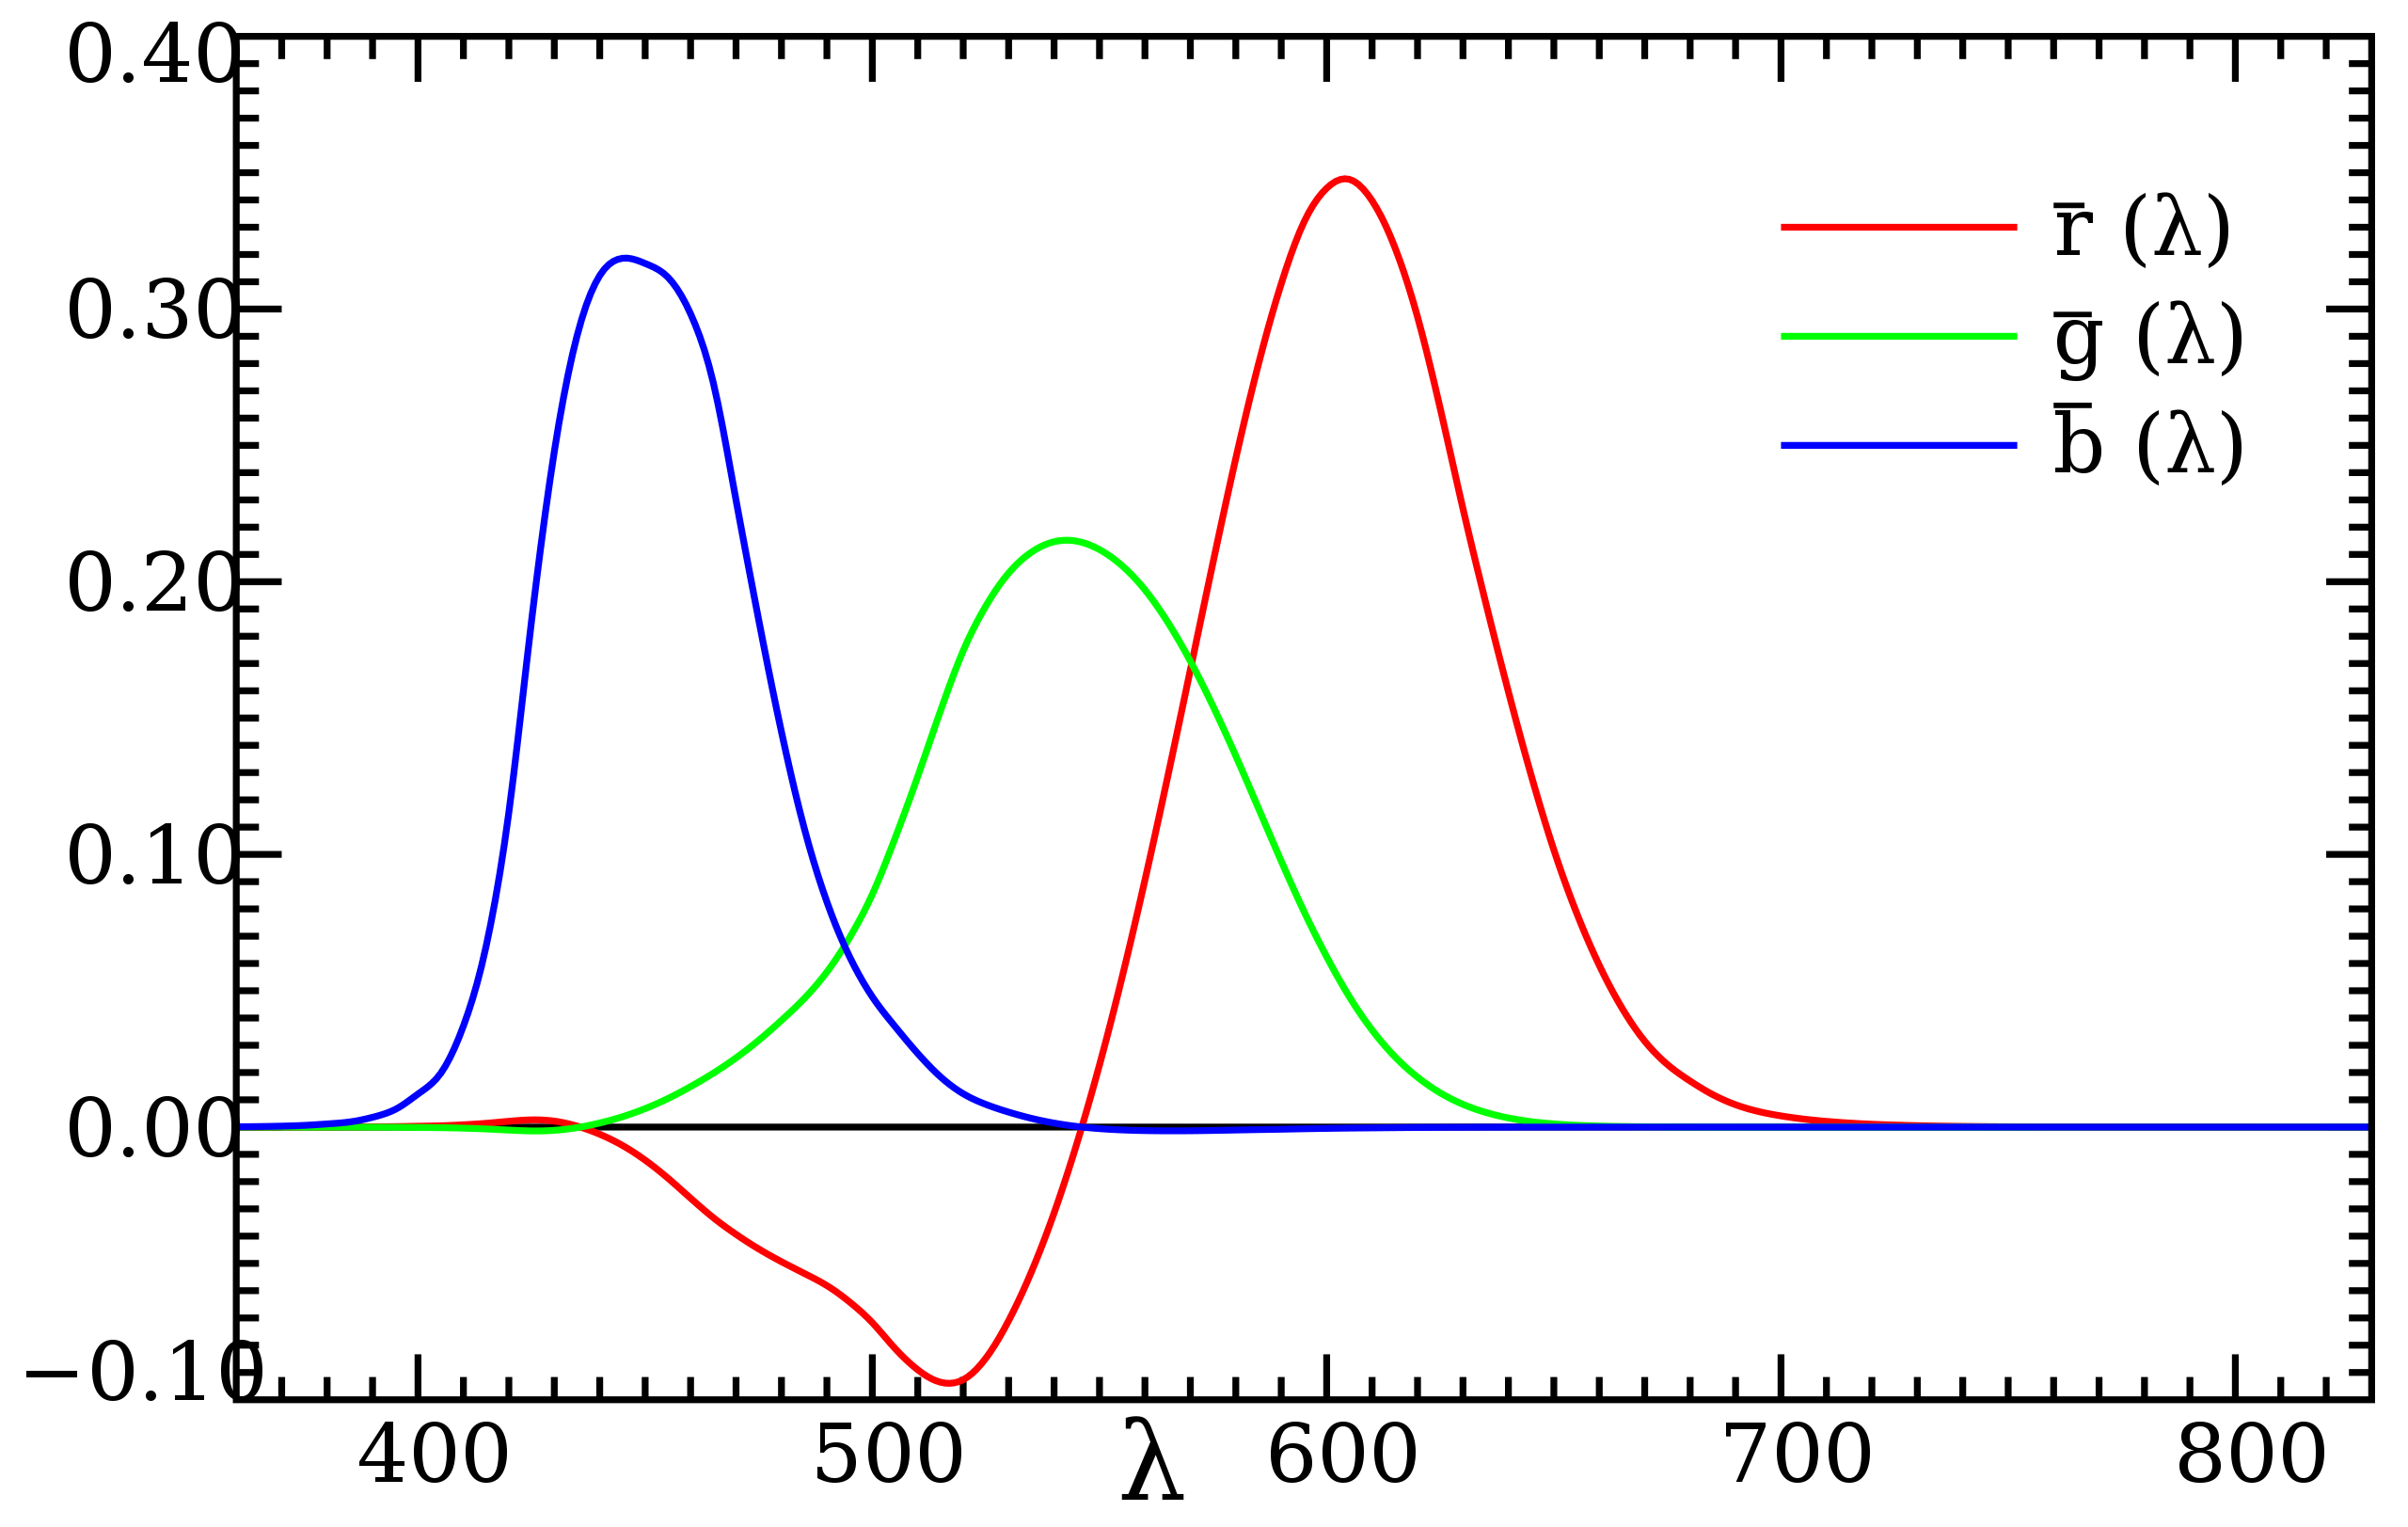
\includegraphics[width=.7\linewidth]{figures/CIE1931_RGBCMF.svg.png}
\end{bonus}

\begin{bonus}[Farbmodell]{CIE 1931-XYZ}
    % TODO: https://de.wikipedia.org/wiki/CIE-Normvalenzsystem#Der_CIE-Normalbeobachter_von_1931_und_1964
    Da negative Werte aus praktischen Gründen (z. B. Rechenschiebern) unerwünscht sind, werden die $\overline{r}$,$\overline{g}$, $\overline{b}$-Farbabgleichsfunktionen linear transformiert.
    Es ergeben sich daraus die $\overline{x}$,$\overline{y}$, $\overline{z}$-\emph{Spektralwertfunktionen}, die den Normalbeobachter charakterisieren.

    Mit Hilfe dieser $\overline{x}$,$\overline{y}$, $\overline{z}$-Spektralwertfunktionen lässt sich die Farbwahrnehmung eines durchschnittlichen Menschen (Normalbeobachter) aus einem gemessenen Lichtspektrum berechnen.
    Dazu werden die Spektralwertfunktionen skalar mit dem gemessenen Lichtspektrum multipliziert.
    Das Ergebnis sind 3 Zahlenwerte:
    (X,Y,Z), wobei Y ein Maß für die Helligkeit liefert.

    Mathematisch gesehen handelt es sich bei der Transformation um eine lineare Koordinatentransformation:
    Aus 3 Werten der $\overline{r}$,$\overline{g}$, $\overline{b}$-Farbabgleichsfunktionen  (R,G,B) die zu der Wellenlänge $\lambda$ gehören, werden mit Hilfe einer Transformationsmatrix die entsprechenden 3 Zahlenwerte (X,Y,Z) der Spektralwertfunktionen im XYZ-Farbraum bestimmt.

    Die Zahlenwerte der Transformationsmatrix sind für diesen Zweck fest vorgegeben:
    \[
        \begin{bmatrix}
            X \\ Y \\ Z
        \end{bmatrix}
        =
        \begin{bmatrix}
            2,768892 & 1,751748 & 1,130160 \\
            1        & 4,590700 & 0,060100 \\
            0        & 0,056508 & 5,594292
        \end{bmatrix}
        \cdot
        \begin{bmatrix}
            R \\ G \\ B
        \end{bmatrix}
    \]

    \centering
    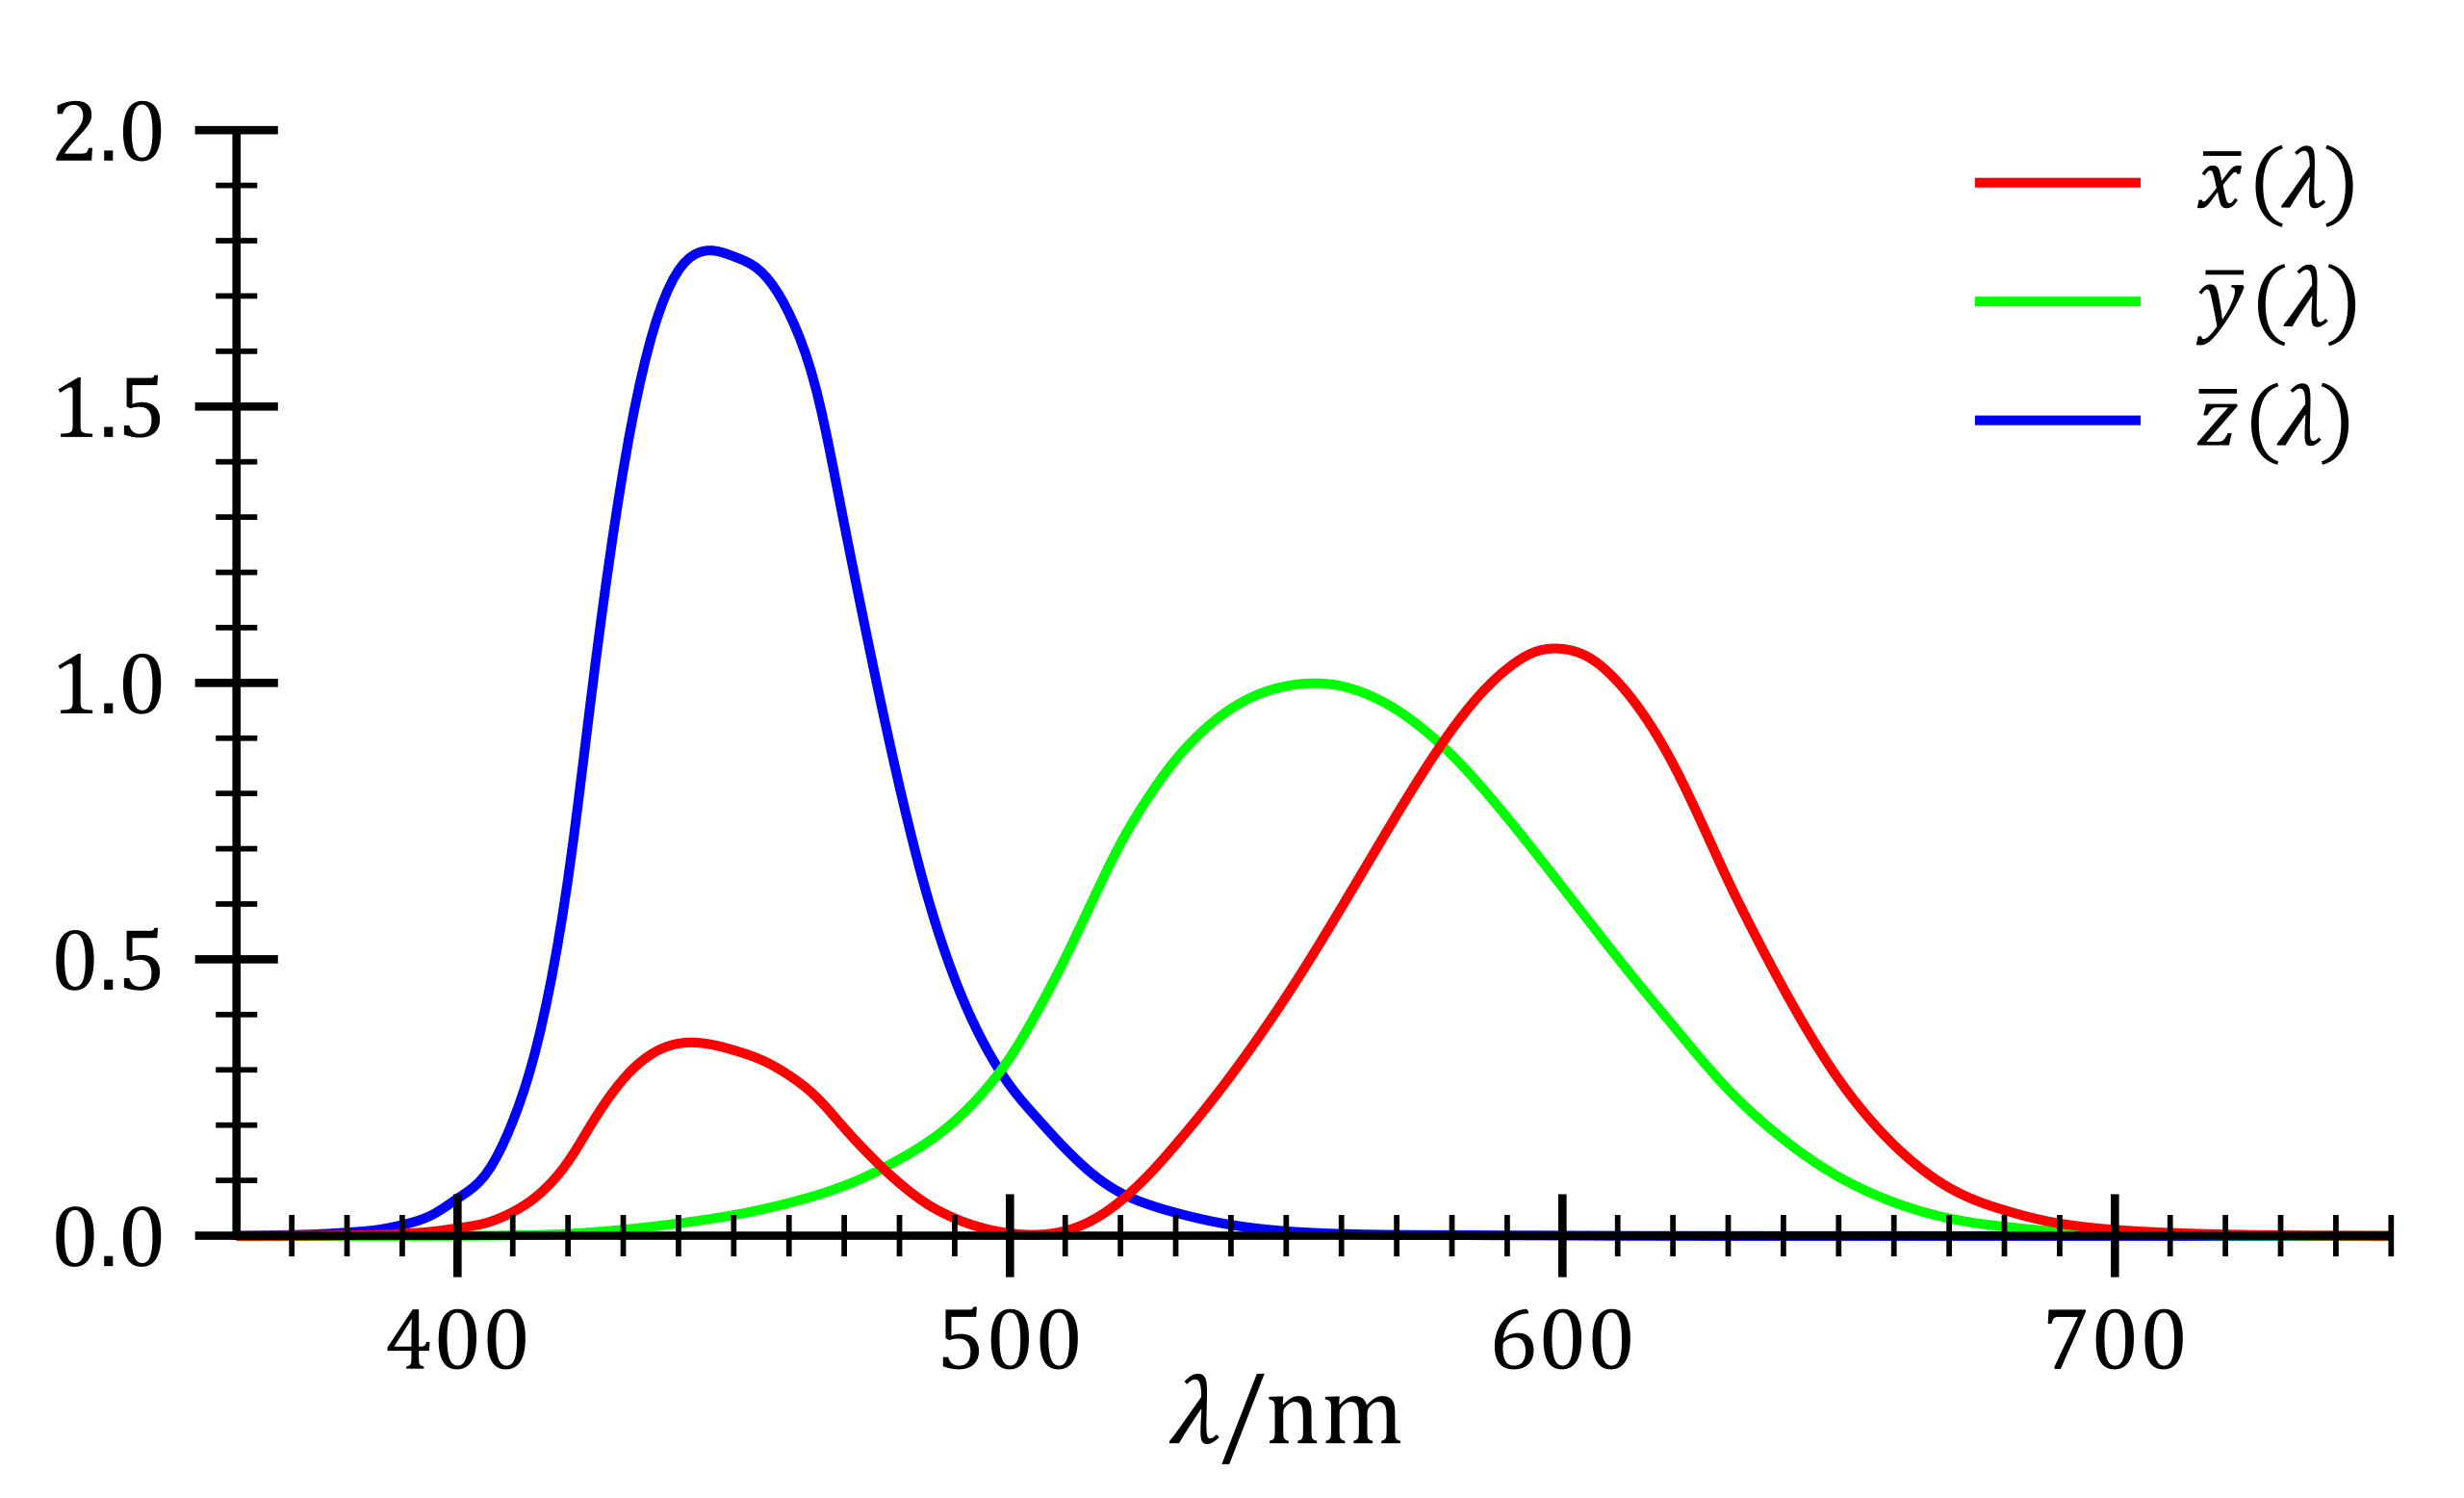
\includegraphics[width=.7\linewidth]{figures/CIE_1931_XYZ_Color_Matching_Functions.png}
\end{bonus}

\begin{bonus}[Farbmodell]{CIE xyY}
    % TODO: https://de.wikipedia.org/wiki/CIE-Normvalenzsystem#Der_CIE-Normalbeobachter_von_1931_und_1964
    Man kann Farbe in Helligkeit und Farbart (Farbton + Farbsättigung) separieren.

    In CIE XYZ ist Y als Helligkeit definiert.
    Umrechnung in \emph{CIE xyY}:
    \[
        x = \frac{X}{X + Y + Z} \quad
        y = \frac{Y}{X + Y + Z} \quad
        z = \frac{Z}{X + Y + Z} = 1 - (x + y)
    \]
    \[
        x + y + z = 1
    \]

    TODO
\end{bonus}

\begin{defi}[Farbmodell]{RGB}
    Ein \emph{RGB-Farbraum} ist ein additiver Farbraum, der Farbwahrnehmungen durch das additive Mischen dreier Grundfarben (Rot, Grün und Blau) nachbildet.
    Das Farbsehen des Menschen ist von drei Zapfentypen geprägt.
    Dieser Farbraum basiert im Prinzip auf der Dreifarbentheorie.

    Der RGB-Farbraum lässt sich als linearer Raum, anschaulich als Farbwürfel, darstellen.

    Die Wertebereiche für die Farbreize (R, G, B) können unterschiedlich festgelegt sein.
    Die klassische Darstellung lässt Werte zwischen 0 und 1 (d. h. 0 Prozent und 100 Prozent) zu;
    dies orientiert sich an der praktischen klassischen Realisierung mittels Dämpfung vorhandenen Lichts.
    Computerorientierte Anwendungen verwenden häufig die an der klassischen Form der Abspeicherung angelehnte Schreibweise, es werden Ganzzahlen zwischen 0 und einer Maximalzahl wie 255 abgespeichert.

    Da die Intensitätswahrnehmung des Menschen nichtlinear ist, wird meist eine nichtlineare Kodierung für die Luminanz vorgenommen. Diese wird häufig als Gamma-Korrektur bezeichnet, da die ersten Implementierungen die Potenzfunktion $Y \sim L^{\frac{1}{\gamma}}$ als Ansatz nutzten.
    Der Koeffizient Gamma mit $\gamma > 1$  beschreibt die Krümmung der Kurve.
    Die inverse Funktion ist $L \sim Y^\gamma$.

    Vorteile:
    \begin{itemize}
        \item RGB ist gut geeignet zum Programmieren von Hardware
    \end{itemize}

    Nachteile:
    \begin{itemize}
        \item Distanz zwischen zwei Punkten entspricht nicht der menschlichen Farbwahrnehmung
        \item Helligkeitsänderungen nicht-linear
        \item Jede Bewegung im Koordinatensystem führt zu einer Änderung von Farbton, Sättigung und Helligkeit (Farbauswahl schwierig und nicht intuitiv)
    \end{itemize}

    \centering
    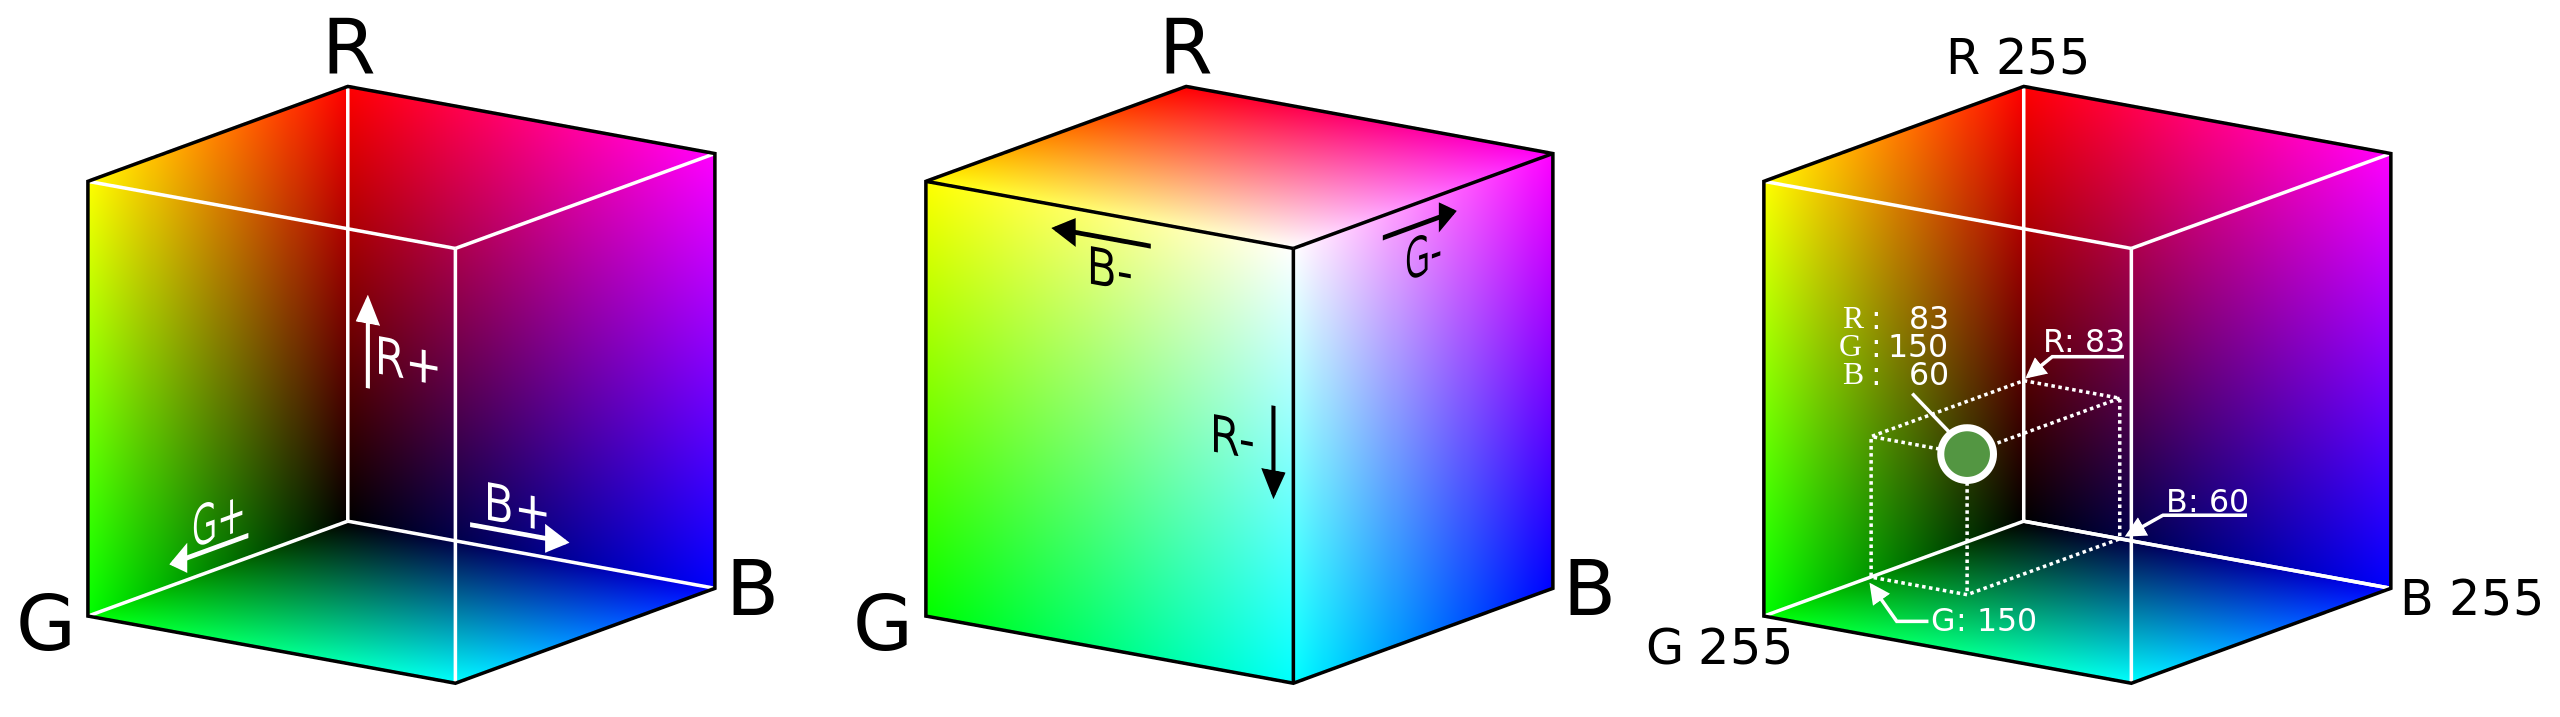
\includegraphics[width=.7\linewidth]{figures/RGB_color_cube.png}
\end{defi}

\begin{defi}{Entsättigung}
    \emph{Entsättigung} ist die gleichmäßige Reduzierung von Farbe.
\end{defi}

\begin{defi}[Farbmodell]{CMYK}
    Das \emph{CMYK-Farbmodell} ist ein subtraktives Farbmodell, das die technische Grundlage für den modernen Vierfarbdruck bildet.
    Die englischsprachige Abkürzung CMYK, die auch in vielen nicht-englischsprachigen Ländern verwendet wird, steht für die drei Farbbestandteile Cyan, Magenta, Yellow und den Schwarzanteil, der traditionell als Key bezeichnet wird.

    Das CMYK-Farbmodell ist ein geräteabhängiges Farbmodell.
    Es beschreibt vordergründig nur, zu welchen Anteilen ein Ausgabegerät die Farbbestandteile kombinieren soll, um einen bestimmten Farbton herzustellen. Wie ein solcher Farbton im Druck aussieht, hängt von der Drucktechnik, den eingesetzten Grundfarben und sogar von der zu bedruckenden Oberfläche ab.

    Die Umrechnung vom RGB-Farbraum zum CMY-Farbraum erfolgt wie folgt:
    \[
        \begin{pmatrix}
            C \\ M \\ Y
        \end{pmatrix}
        =
        \begin{pmatrix}
            1 - R \\
            1 - G \\
            1 - B
        \end{pmatrix}
    \]

    Die zusätzliche Druckfarbe Schwarz (Key), für die das CMYK-Farbmodell entworfen wurde, ist für den Zusammendruck der drei Bunttöne nötig, da diese theoretisch, aber nicht praktisch ein ausreichend tiefes Schwarz ergeben.
    Um CMY in CMYK umzurechnen gibt es verschiedene Varianten, z. B.:
    \begin{itemize}
        \item lineare Reduktion der Farben mit wachsendem $K$:
              \[
                  \begin{pmatrix}
                      C' \\ M' \\ Y' \\ K'
                  \end{pmatrix}
                  =
                  \begin{pmatrix}
                      C - K \\
                      M - K \\
                      Y - K \\
                      K
                  \end{pmatrix}
              \]
        \item stärkere Farben in dunklen Bereichen:
              \[
                  \begin{pmatrix}
                      C' \\ M' \\ Y' \\ K'
                  \end{pmatrix}
                  =
                  \begin{pmatrix}
                      (C - K) \cdot s \\
                      (M - K) \cdot s \\
                      (Y - K) \cdot s \\
                      K
                  \end{pmatrix}
                  , \quad s \begin{cases}
                      \frac{1}{1 - K} & K < 1        \\
                      1               & \text{sonst}
                  \end{cases}
              \]
    \end{itemize}
\end{defi}

\begin{defi}[Farbmodell]{HSV}
    % TODO: https://de.wikipedia.org/wiki/HSV-Farbraum
    Der \emph{HSV-Farbraum} ist der Farbraum etlicher Farbmodelle.
    Hier ist der Farbort einer Farbe definiert mit Hilfe der drei Koordinaten:
    \begin{itemize}
        \item Farbwert (englisch hue): Farbwinkel auf dem Farbkreis (0° für Rot, 120° für Grün, 240° für Blau)
        \item Farbsättigung (saturation): (0 \% = Neutralgrau, 50 \% = wenig gesättigte Farbe, 100 \% = gesättigte, reine Farbe)
        \item Hellwert (value; auch Dunkelstufe genannt): (0 \% = keine Helligkeit, 100 \% = volle Helligkeit)
    \end{itemize}

    In Fragen der Farbnachstellung wird das HSV-Modell gegenüber den Alternativen RGB und CMYK bevorzugt, weil es der menschlichen Farbwahrnehmung stärker entspricht (beispielsweise ist es im RGB-Modell schwer, sich Gelb als Mischung von Rot und Grün vorzustellen).
    Für die Farbmischung kann man unmittelbar den gewünschten Farbton wählen und dann entscheiden, wie gesättigt und wie hell (oder dunkel) dieser sein soll, oder ob eine andere Farbnuance passender ist:

    Der Farbwinkel spezifiziert die dominante Wellenlänge der Farbe, mit Ausnahme des Bereiches zwischen Blauviolett und Rot (240° und 360°), wo er eine Position auf der Purpurlinie angibt.

    Die Sättigung entspricht der Zumischung von purem Weiß (d. h. Licht mit gleichen Intensitäten in allen Wellenlängen) zu einer simulierten Spektralfarbe (oder vielmehr der entsprechenden Spaltbreite um die dominante Wellenlänge herum);
    dabei entspricht stärkere Weiß-Zumischung einer geringeren Sättigung.

    Die Helligkeit ist ein Parameter für den Gesamtenergieinhalt bzw. für die maximale Amplitude des Lichts;
    die Dunkelstufe ergänzt diesen Wert im Gegensätzlichen.
    Nachteilig bei der Dunkelstufe ist, dass Weiß und ein beliebiger Farbton die gleiche Sättigung haben können.

    In diesem System wird Weiß als Buntfarbe behandelt.
    In der Praxis wiederum ist die Umwandlung eines Farbbildes in ein Schwarz-Weiß-Bild durch Ändern nur einer Koordinate nicht möglich.

    \centering
    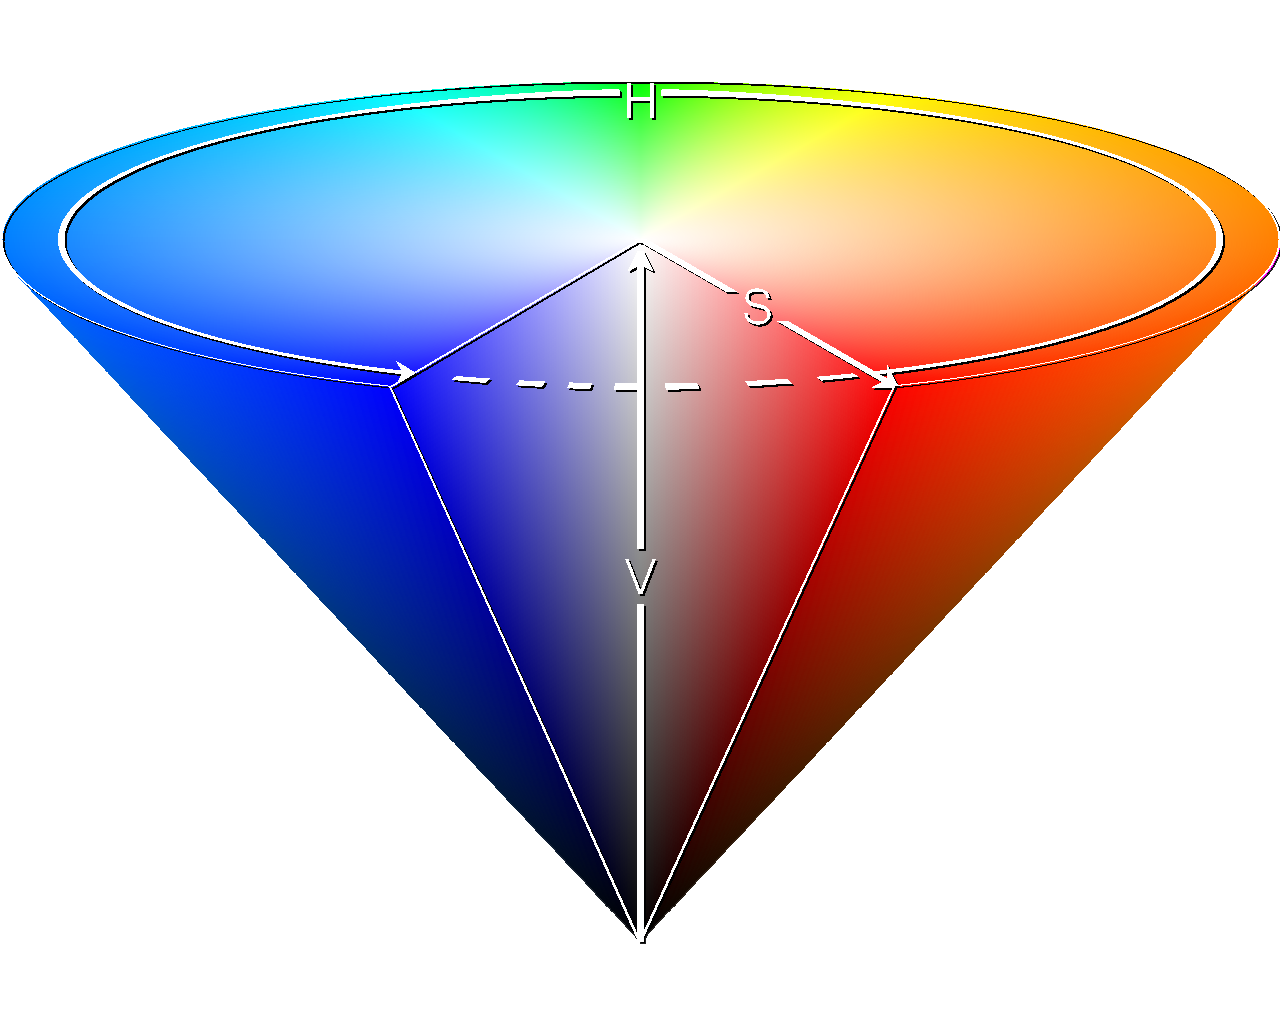
\includegraphics[width=.4\linewidth]{figures/HSV_cone.png}
\end{defi}

\begin{defi}[Farbmodell]{HSI}
    An den Bedürfnissen der Farbmetrik und der phototechnischen Reproduktion orientiert sich das \emph{HSI-Modell}.
    Auch hierbei steht H für Buntwert (hue) und S für Sättigung.

    Der Unterschied bezieht sich auf die dritte Koordinate, die Lichtintensität I.

    TODO: Umrechnung
\end{defi}

\begin{bonus}[Farbmodell]{HSL}
    Der \emph{HSL-Farbraum} hat die Parameter Farbwinkel $H$, Farbsättigung $S$ und Farbhelligkeit $L$.

    Im Gegensatz zum HSV-Farbraum wird er jedoch auf den zwischen Weiß und Schwarz liegenden Graupunkt als neutrales Grau bezogen.
    Der Graupunkt liegt in der Mitte und die Buntwerte außen, der Farbkörper wird daher als Doppelkegel, (Doppel-)Zylinder oder sechsseitiges Prisma dargestellt.

    \centering
    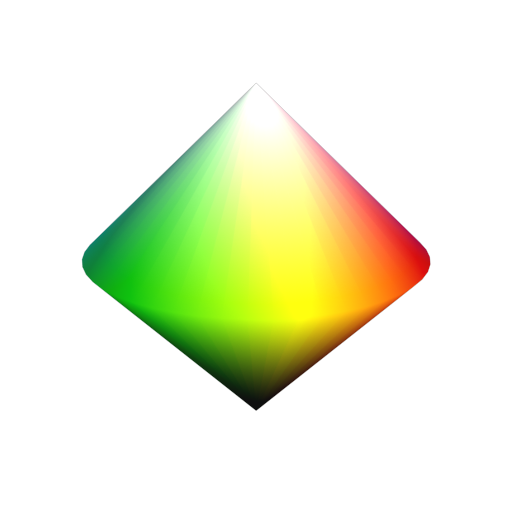
\includegraphics[width=.4\linewidth]{figures/HSL_cone.png}
\end{bonus}

\begin{defi}[Farbmodell]{YUV}
    % TODO: https://de.wikipedia.org/wiki/YUV-Farbmodell 
    Das \emph{YUV-Farbmodell} wird beim analogen Farbfernsehen nach den Normen PAL und NTSC verwendet.

    Es verwendet zur Darstellung der Farbinformation zwei Komponenten:
    \begin{itemize}
        \item die Luminanz (luma, Lichtstärke pro Fläche, d. h. Leuchtdichte) $Y$ und
        \item die Chrominanz (Farbanteil, chroma), wobei diese aus den zwei Unterkomponenten $U$ und $V$ besteht.
    \end{itemize}

    Wie das Farbdreieck, von dem es abgeleitet wurde, geht das YUV-Farbmodell von einem Modell mit linearer Addition der Farbreize aus.
    Diese Modelle sind mit Hilfe einer Matrix ineinander überführbar.

    Zur Berechnung des Luma-Signals $Y$ werden die zugrundeliegenden RGB-Daten zunächst mit dem Gamma-Wert des Ausgabegerätes verrechnet;
    man erhält ein $R'G'B'$-Signal.
    Die drei Einzelkomponenten werden mit unterschiedlicher Gewichtung addiert, um die Helligkeitsinformation zu bilden.

    Die Gewichtung der Komponenten ist erforderlich, da einige Aspekte des Farbensehens des menschlichen Auges berücksichtigt werden müssen.
    So wird beispielsweise Grün heller wahrgenommen als Rot, dieses wiederum heller als Blau.
    Diese unterschiedliche Gewichtung wird in folgender (per Definition exakten) Umrechnungsformel berücksichtigt:
    \[
        Y := 0.299 \cdot R + 0.587 \cdot G + 0.114 \cdot B
    \]

    Die \emph{Chrominanzsignale} (auch Farbdifferenzsignale) $U$ und $V$ enthalten die Farbinformation. Sie entstehen aus der Differenz zwischen Blauanteil B und Luminanz Y bzw. zwischen Rotanteil und Luminanz sowie einer weiteren Reduktion;
    auch diese Formeln sind per Definition exakt:
    \[
        U := 0.493 \cdot (B - Y)
    \]
    \[
        V := 0.877 \cdot (R - Y)
    \]

    Aus den drei erzeugten Komponenten $Y$, $U$ und $V$ können später wieder die einzelnen Farbanteile der Grundfarben berechnet werden durch die jeweiligen Rücktransformationen.

    \centering
    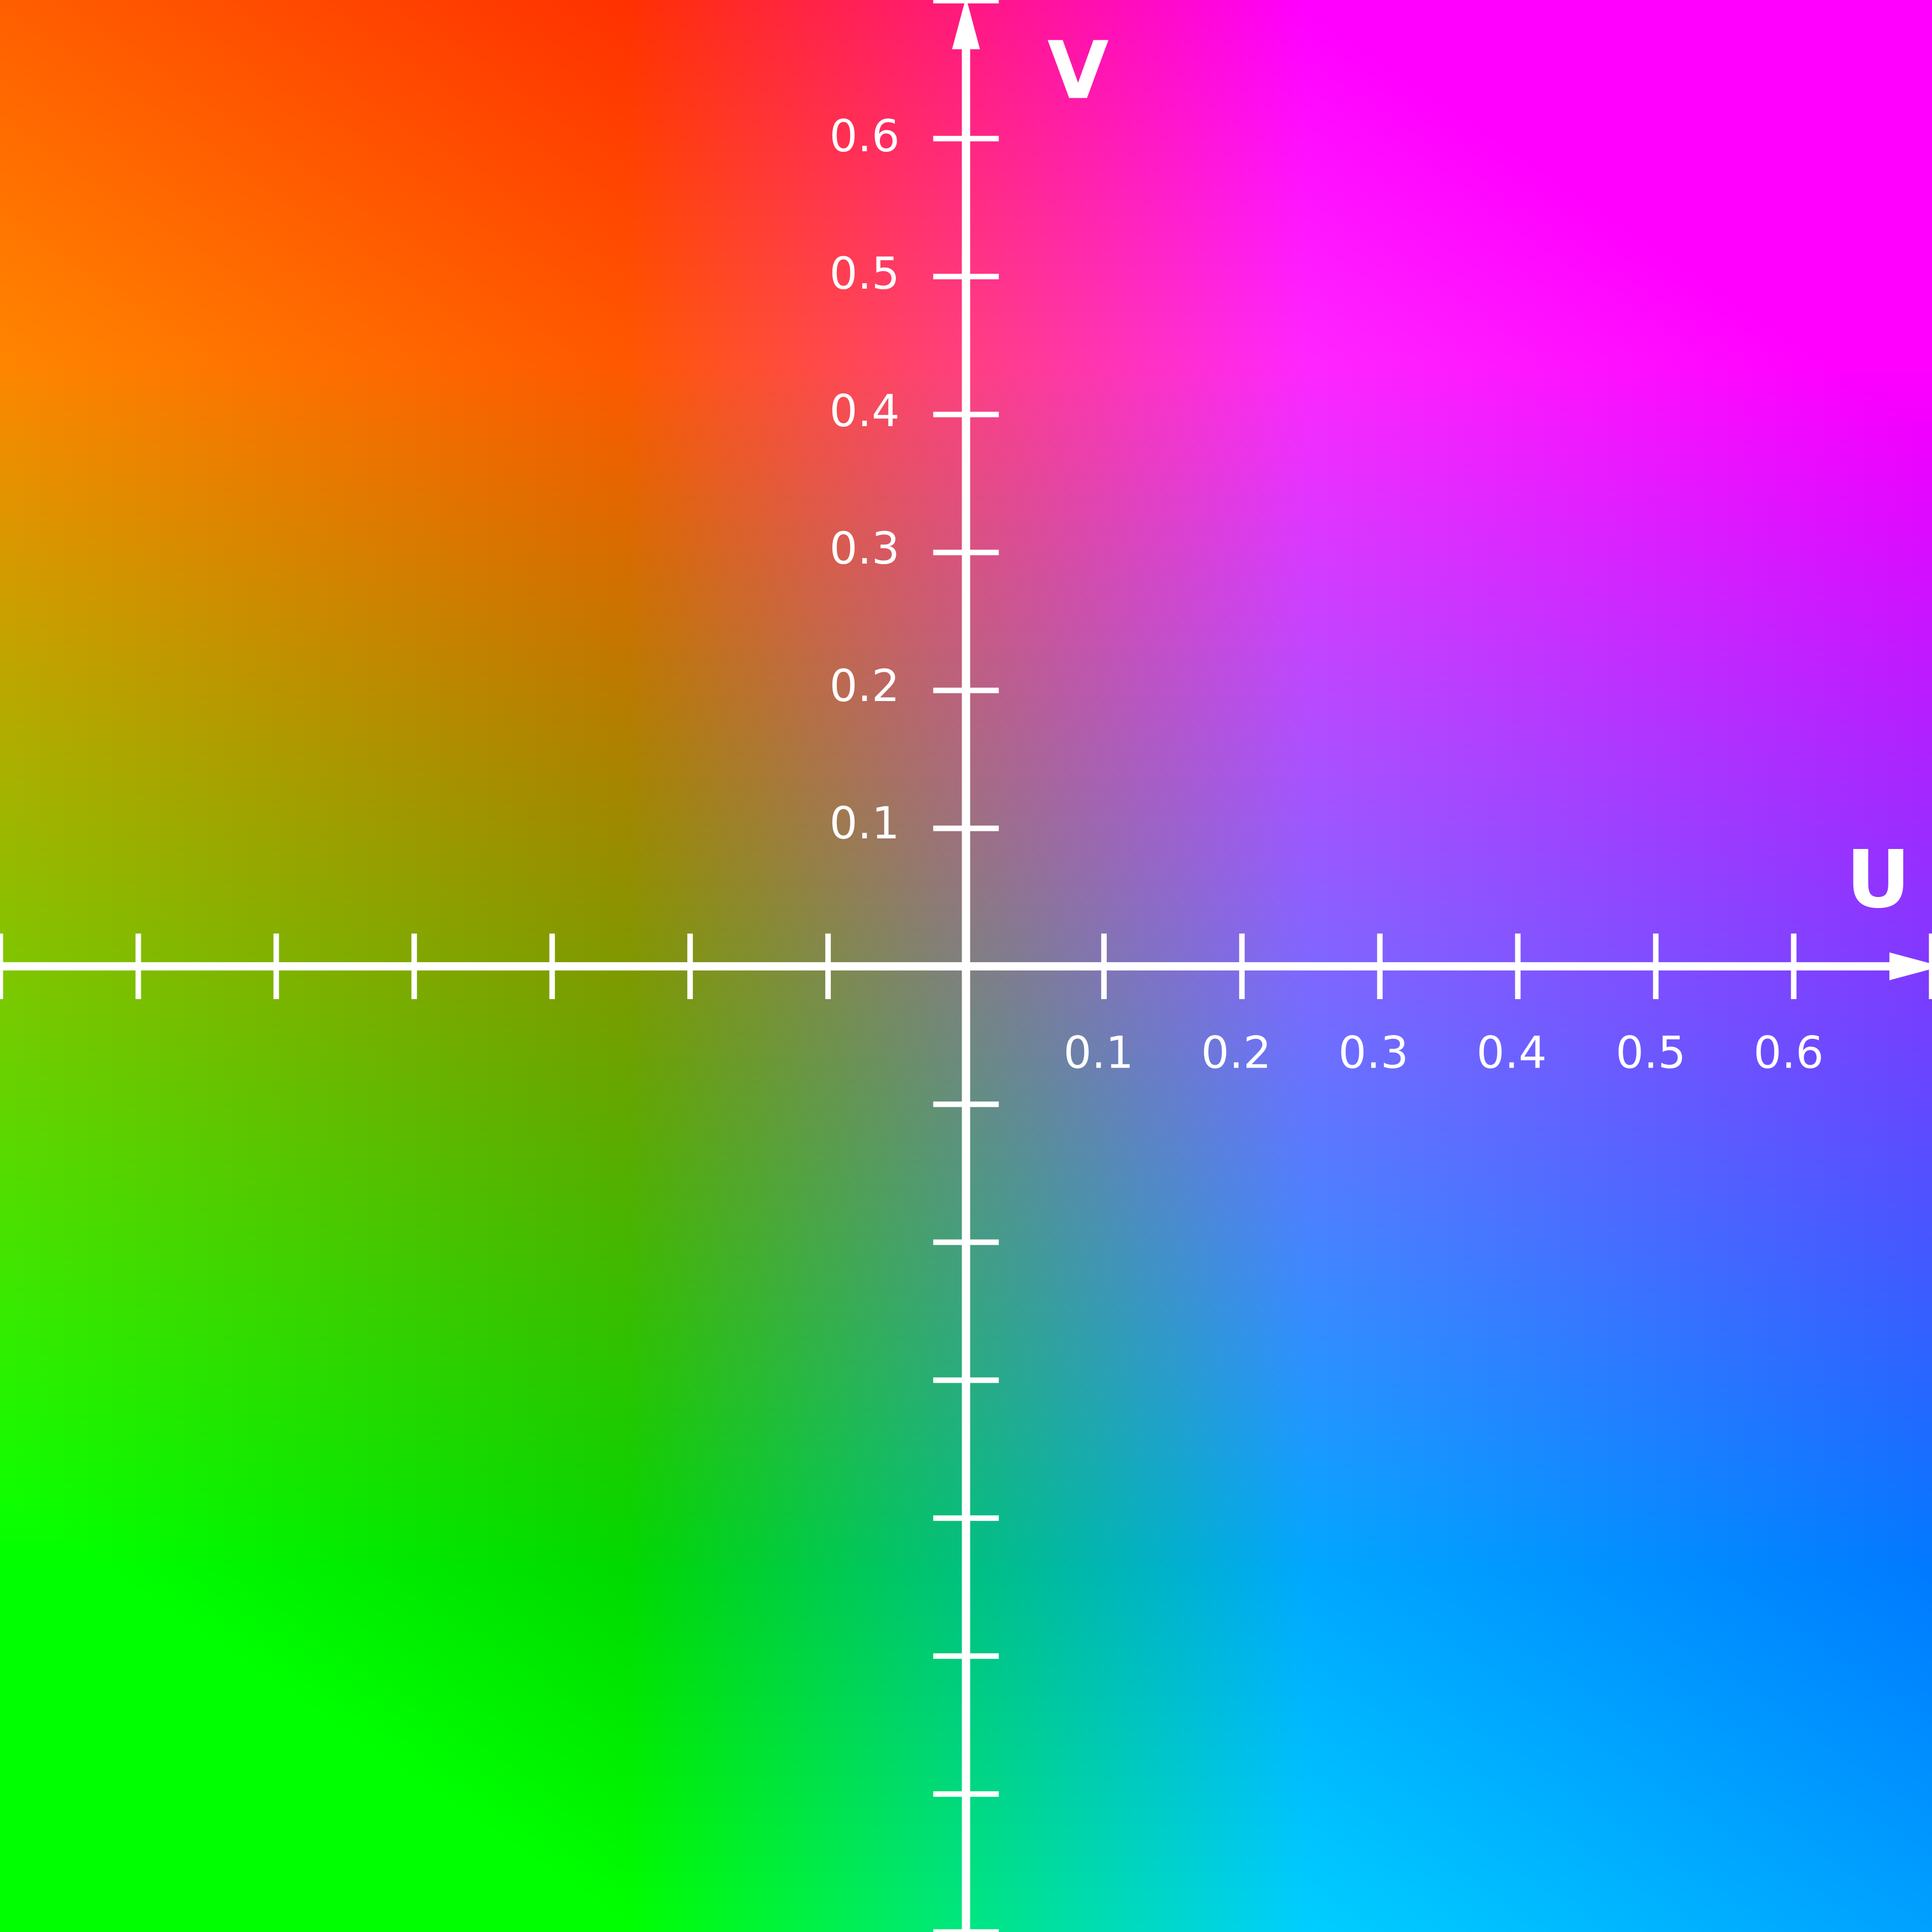
\includegraphics[width=.4\linewidth]{figures/YUV-UV_Scaled_Y0.5_70_percent.png}

    UV-Fläche des YUV-Farbmodells im RGB-Farbraum auf einer Helligkeitsebene von $Y = 0.5$.
\end{defi}

\begin{defi}[Farbmodell]{YCbCr}
    % TODO: https://de.wikipedia.org/wiki/YCbCr-Farbmodell
    Das \emph{YCbCr-Farbmodell} wurde für das Digitalfernsehen nach der Norm PAL entwickelt, wird heute aber auch beim digitalen NTSC-Fernsehen genutzt.

    Das YCbCr-Modell teilt die Farbinformation in die Grundhelligkeit $Y$ und die zwei Farbkomponenten $Cb$ (Blue-Yellow Chrominance) und $Cr$ (Red-Green Chrominance) auf.
    Mit $Y$ wird hier die Helligkeitsachse aus dem CIE-Normvalenzsystem verwendet.
    Sie entspricht der Hellempfindlichkeit des Auges, die im grünen Spektralbereich am größten ist.
    Chrominance oder kurz Chroma bedeutet Buntheit im Allgemeinen und Farbigkeit in Bezug auf Helligkeit-Farbigkeits-Modelle.

    Vergleicht man die beiden Separationen des Bildbeispiels in YUV und YCbCr, wird ersichtlich, dass der Helligkeitskanal ein völlig unbuntes Graustufenbild zeigt und, dass lediglich die Chrominanzachsen U und V in der Farbtafel andere Farbtöne durchschneiden als Cb und Cr.
    Cb ist also ein Maß für die Abweichung der Farbigkeit von Grau in Richtung Blau/Gelb, Cr ist die entsprechende Maßzahl in Richtung Rot/Türkis.

    \centering
    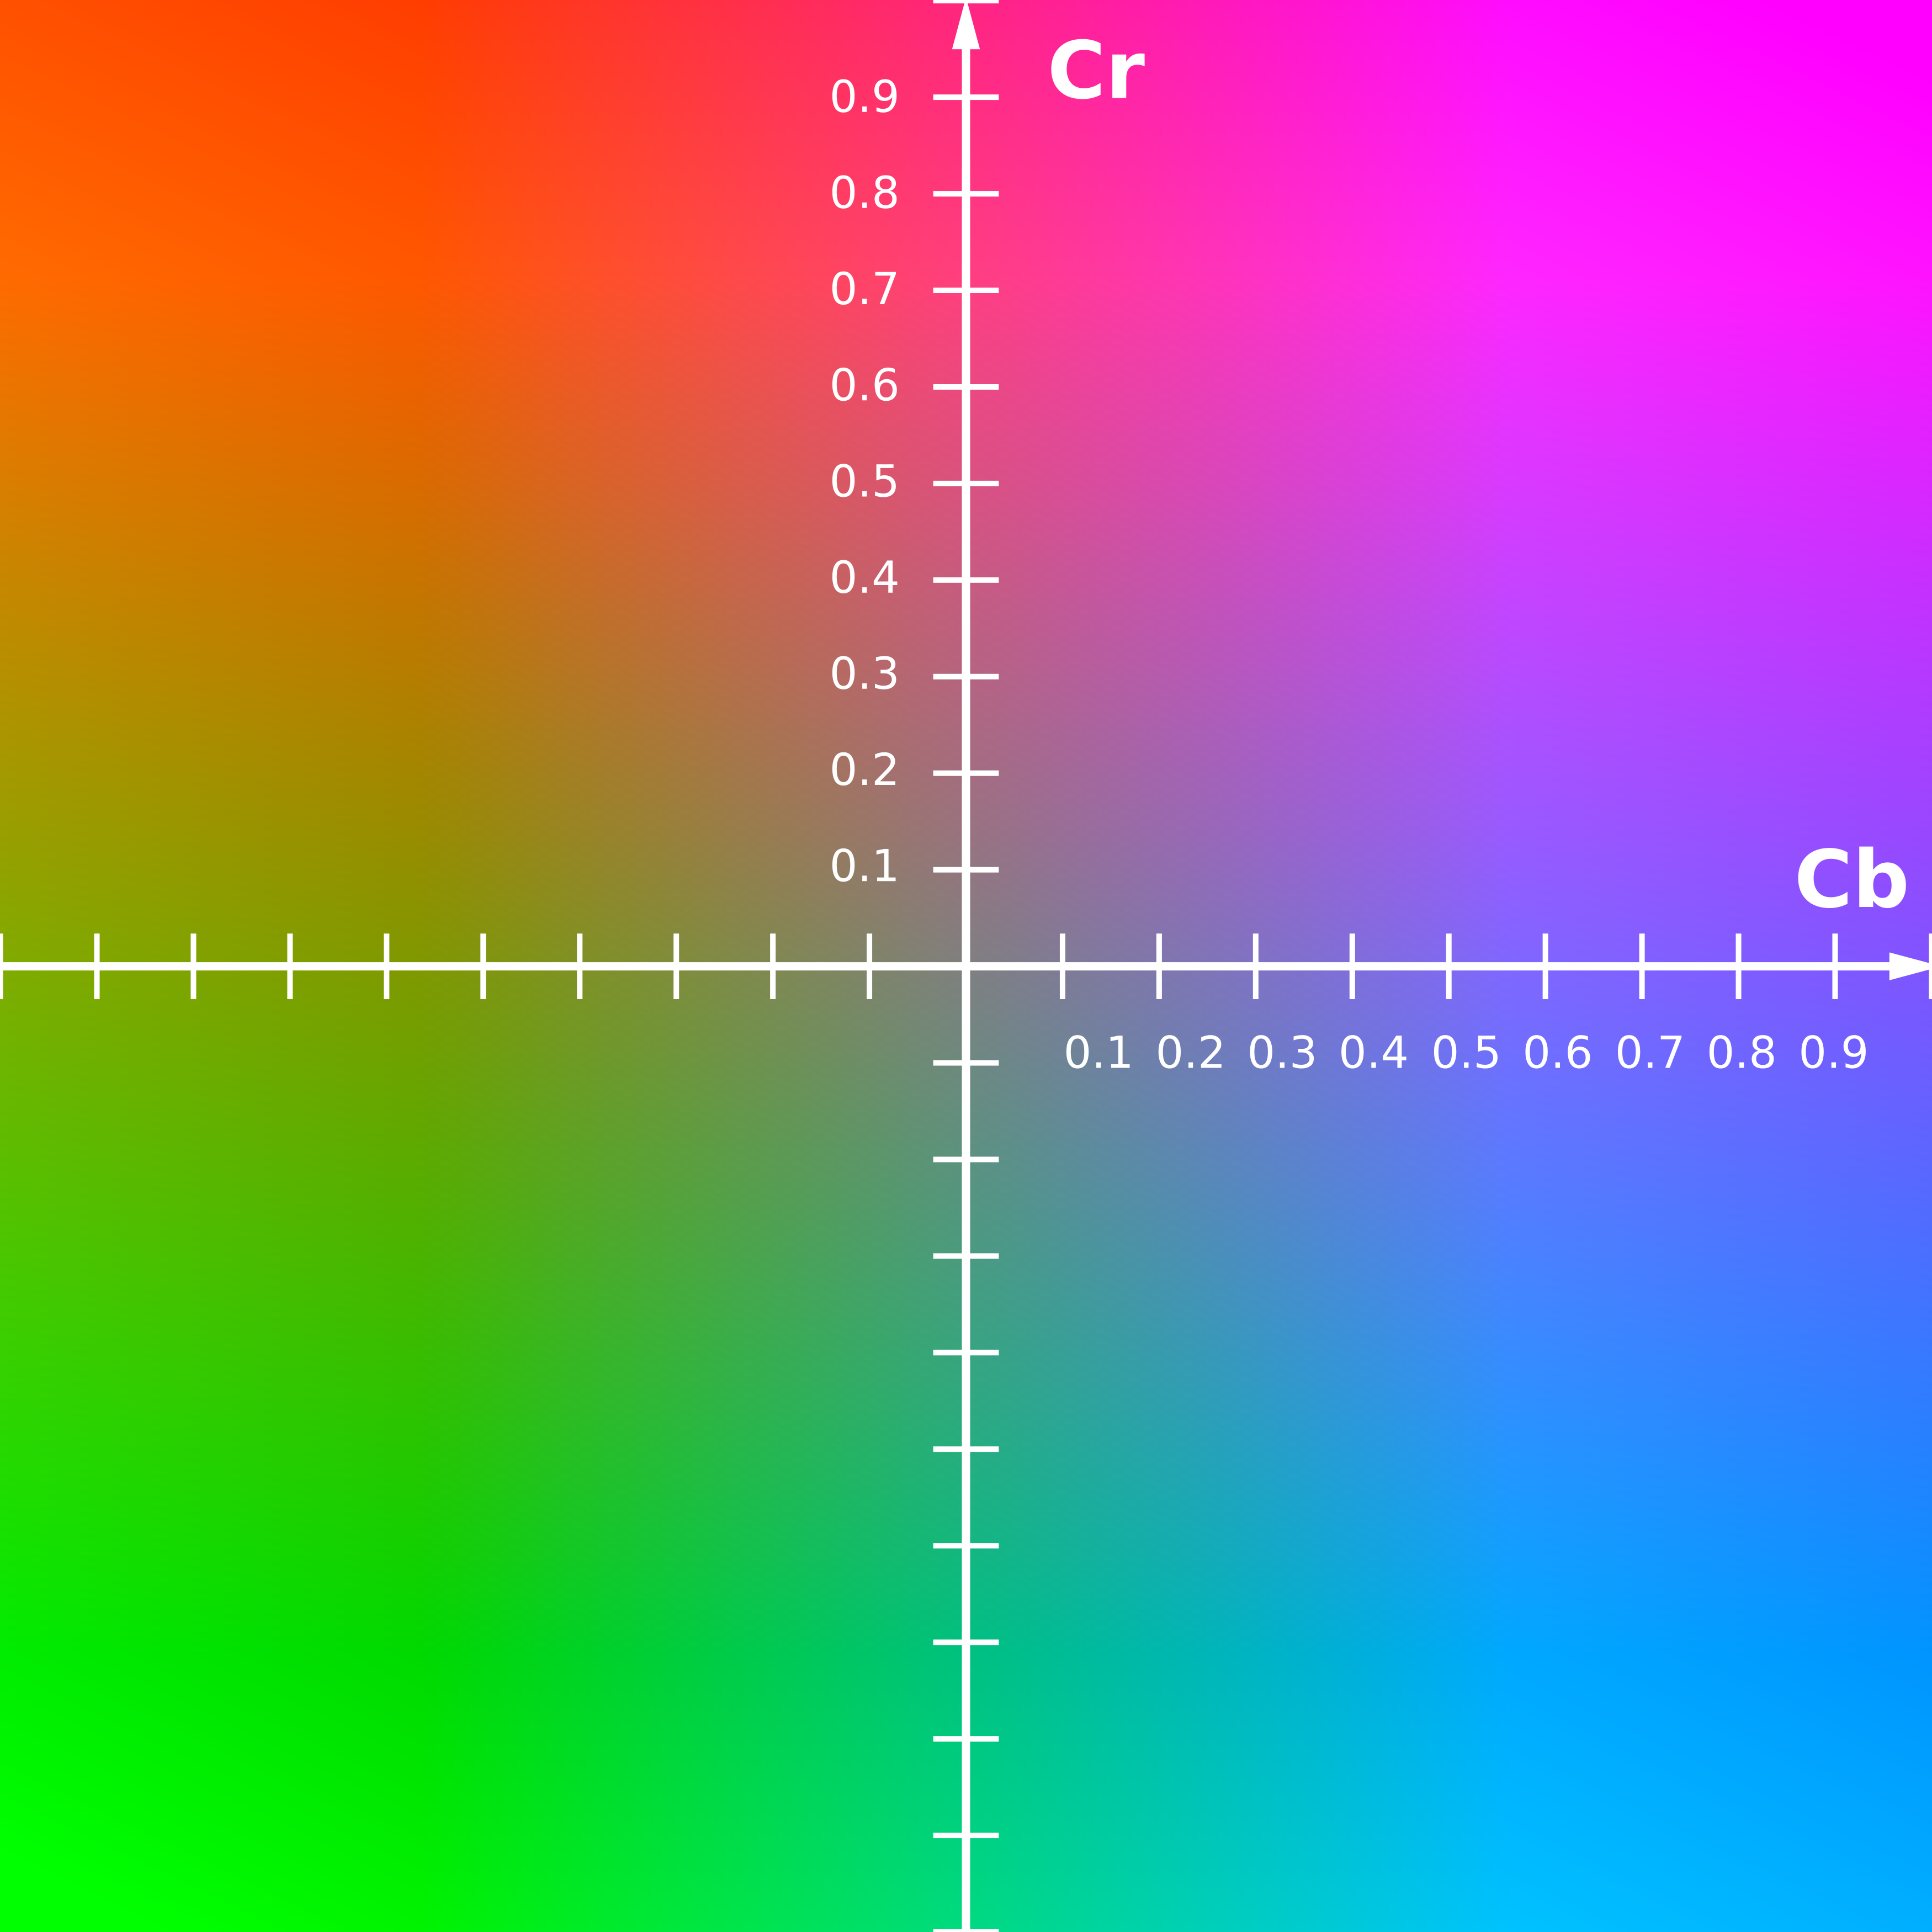
\includegraphics[width=.4\linewidth]{figures/YCbCr-CbCr_Scaled_Y50.png}

    CbCr-Fläche des YCbCr-Farbmodells im RGB-Farbraum auf einer Helligkeitsebene von $Y = 0.5$.
\end{defi}

\begin{bonus}[Farbmodell]{CIE L*a*b*}
    TODO
\end{bonus}

\begin{bonus}[Farbmodell]{CIE LCh}
    TODO
\end{bonus} % VL 06

% Until 06/30/2023
% \section{Evaluation von Segmentierungsergebnissen}

\begin{defi}{Metrik}
    % TODO: https://de.wikipedia.org/wiki/Metrischer_Raum#Einordnung_in_die_Hierarchie_mathematischer_Strukturen 
    Sei $X$ eine beliebige Menge.
    Eine Abbildung $d: X \times X \to \mathbb {R}$ heißt \emph{Metrik} auf $X$, wenn für beliebige Elemente $x, y, z \in \mathbb{R}$ die folgenden Eigenschaften gelten:
    \begin{itemize}
        \item Positive Definitheit: $d(x, y) \geq 0$ und $d(x, y) = 0 \iff x = y$.
        \item Symmetrie: $d(x, y) = d(y, x)$
        \item Dreiecksungleichung: $d(x, y) \leq d(x, z) + d(z, y)$
    \end{itemize}
\end{defi}

\begin{defi}{Wahrheitsmatrix}
    % TODO: https://de.wikipedia.org/wiki/Beurteilung_eines_bin%C3%A4ren_Klassifikators#Wahrheitsmatrix:_Richtige_und_falsche_Klassifikationen 
    Um einen Klassifikator zu bewerten, muss man ihn in einer Reihe von Fällen anwenden, bei denen man zumindest im Nachhinein Kenntnis über die \enquote{wahre} Klasse der jeweiligen Objekte hat.
    Dabei können vier mögliche Fälle auftreten:
    \begin{itemize}
        \item \emph{Richtig positiv} (engl. true positive, \emph{TP})
        \item \emph{Falsch negativ} (engl. false negative, \emph{FN})
        \item \emph{Falsch positiv} (engl. false positive, \emph{FP})
        \item \emph{Richtig negativ} (engl. true negative, \emph{TN})
    \end{itemize}

    Es wird nun gezählt, wie häufig jede der vier möglichen Kombinationen von ermittelter Klasse und tatsächlicher Klasse vorgekommen ist.
    Diese Häufigkeiten werden in eine sogenannte \emph{Wahrheitsmatrix} (auch Konfusionsmatrix genannt) eingetragen:

    TODO: Tabelle

    \centering
    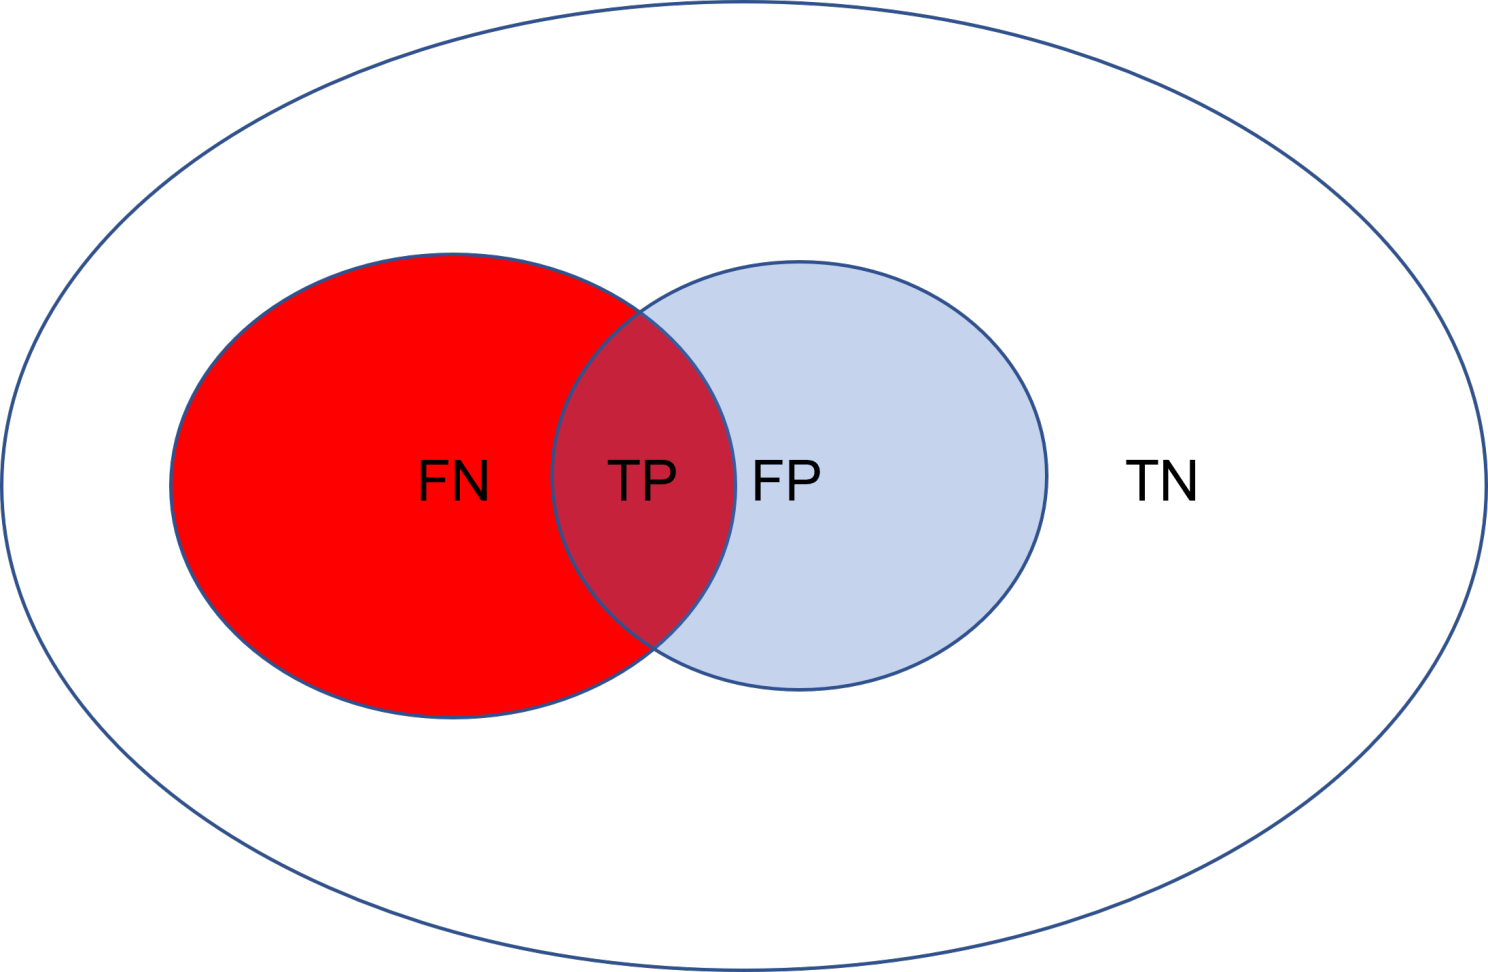
\includegraphics[width=.5\linewidth]{figures/wahrheitsmatrix_venn.png}
\end{defi}

\begin{defi}[Überlappungsmetrik]{Jaccard-Koeffizient}
    % TODO: https://de.wikipedia.org/wiki/Jaccard-Koeffizient 
    Der \emph{Jaccard-Koeffizient} oder \emph{Jaccard-Index}, auch \emph{Intersection over Union} ist eine Kennzahl für die Ähnlichkeit von Mengen.

    Um den Jaccard-Koeffizient zweier Mengen zu berechnen, teilt man die Anzahl der gemeinsamen Elemente (Schnittmenge) durch die Größe der Vereinigungsmenge:
    \[
        J(A, B) = \frac{|A \cap B|}{|A \cup B|}
    \]
    Je näher der Jaccard-Koeffizient an $1$ liegt, desto größer ist die Ähnlichkeit der Mengen.
    Der minimale Wert des Jaccard-Koeffizienten ist $0$.
\end{defi}

\begin{bonus}[Überlappungsmetrik]{DICE-Koeffizient}
    Der \emph{DICE-Koeffizient} berechnet sich als zweimal die Schnittmenge geteilt durch die Summe der Kardinalitäten der einzelnen Mengen.
    \[
        D(A, B) = \frac{2 \cdot |A \cap B|}{|A| +  |B|}
    \]

    DICE lässt sich in Jaccard ausdrücken und umgekehrt.
    Beide Metriken messen die gleichen Aspekte.
\end{bonus}

\begin{defi}[Überlappungsmetrik]{Sensitivität}
    Die \emph{Sensitivität} (auch \emph{Richtig-positiv-Rate}; engl. \emph{Sensitivity}, \emph{True Positive Rate}, \emph{Recall} oder \emph{Hit Rate}) gibt die Wahrscheinlichkeit an, mit der ein positives Objekt korrekt als positiv klassifiziert wird.

    Beispielsweise bedeutet eine Sensitivität eines Tests auf ein Virus von 98 \%, dass (bei ausreichend großer Anzahl an durchgeführten Tests und unabhängig von den Testvorbedingungen) 98 \% der Infizierten erkannt und 2 \% der Infizierten nicht erkannt würden.
    2 \% (der Infizierten, welche getestet wurden, und nicht aller Getesteten) wären dann also falsch negativ.

    Die Sensitivität entspricht der geschätzten bedingten Wahrscheinlichkeit:
    \[
        \text{Sensitivity} = P(\text{positives Testergenis} \mid \text{tatsächlich krank}) = \text{TPR} = \frac{\text{TP}}{\text{TP} + \text{FN}}
    \]

    Die Sensitivität ist empfindlich bzgl. der Größe der Ergebnismengen.
    Fehler in kleinen Ergebnismengen werden stärker betont, als in großen Ergebnismengen.

    TODO: Venn-Diagramm
\end{defi}

\begin{defi}[Überlappungsmetrik]{Spezifizität}
    Die \emph{Spezifität} (auch \emph{Richtig-negativ-Rate}; engl. \emph{Specificity}, \emph{True Negative Rate}) gibt die Wahrscheinlichkeit an, mit der ein negatives Objekt korrekt als negativ klassifiziert wird.

    % Beispielsweise entspricht die Spezifität bei einer medizinischen Diagnose dem Anteil an Gesunden, bei denen auch festgestellt wurde, dass keine Krankheit vorliegt. 
    % Die Spezifität eines Tests gibt an, mit welcher Wahrscheinlichkeit ein Nicht-Infizierter auch tatsächlich erkannt würde. 

    Beispielsweise bedeutet eine Spezifität eines Tests auf ein Virus von 98 \%, dass (bei ausreichend großer Anzahl an durchgeführten Tests und unabhängig von den Testvorbedingungen) 98 \% der Nicht-Infizierten tatsächlich erkannt und 2 \% der Nicht-Infizierten fälschlich als infiziert ausgewiesen würden.
    2 \% (der getesteten Nicht-Infizierten, nicht der Getesteten insgesamt) wären dann also falsch positiv.

    Die Spezifität entspricht der geschätzten bedingten Wahrscheinlichkeit:
    \[
        \text{Specificity} = P(\text{negatives Testergenis} \mid \text{tatsächlich gesund}) = \text{TNR} = \frac{\text{TN}}{\text{TN} + \text{FP}}
    \]

    Die Spezifizität ist empfindlich bzgl. der Größe der Ergebnismengen.
    Fehler in kleinen Ergebnismengen werden stärker betont, als in großen Ergebnismengen.

    TODO: Venn-Diagramm
\end{defi}

\begin{bonus}[Überlappungsmetrik]{False-positiv-Rate}
    Die \emph{Falsch-positiv-Rate} lässt sich aus der Spezifizität ableiten:
    \[
        FPR = 1 - \text{Specificity} = \frac{\text{FP}}{\text{FP} + \text{TN}}
    \]

    TODO: Venn-Diagramm
\end{bonus}

\begin{bonus}[Überlappungsmetrik]{False-negativ-Rate}
    Die \emph{Falsch-negativ-Rate} lässt sich aus der Sensitivität ableiten:
    \[
        FNR = 1 - \text{Sensitivity} = \frac{\text{FN}}{\text{FN} + \text{TP}}
    \]

    TODO: Venn-Diagramm
\end{bonus}

\begin{defi}[Überlappungsmetrik]{Positive Predictive Value}
    Der \emph{positive Vorhersagewert} (engl. \emph{Positive Predictive Value}, \emph{PPV}) gibt den Anteil der korrekt als positiv klassifizierten Ergebnisse an der Gesamtheit der als positiv klassifizierten Ergebnisse an:
    \[
        \text{Specificity} = \text{PPV} = \frac{\text{TP}}{\text{TP} + \text{FP}}
    \]
\end{defi}

\begin{defi}[Überlappungsmetrik]{Negative Predictive Value}
    Der \emph{negative Vorhersagewert} (engl. \emph{Negative Predictive Value}, \emph{NPV}) gibt den Anteil der korrekt als negativ klassifizierten Ergebnisse an der Gesamtheit der als negativ klassifizierten Ergebnisse an:
    \[
        \text{NPV} = \frac{\text{TN}}{\text{TN} + \text{FN}}
    \]
\end{defi}

\begin{defi}[Entfernungsmetrik]{Hausdorff-Distanz}
    % TODO: https://de.wikipedia.org/wiki/Hausdorff-Metrik
    Die \emph{(symmetrische) Hausdorff-Distanz} misst den Abstand $\delta(A, B)$ zwischen nichtleeren kompakten Teilmengen $A$, $B$ eines metrischen Raums $E$.

    Anschaulich haben zwei kompakte Teilmengen einen geringen Hausdorff-Abstand, wenn es zu jedem Element der einen Menge ein Element der anderen Menge gibt, zu dem dieses einen geringen Abstand hat.

    Als Hilfsmittel definiert man den Abstand $D$ zwischen einem Punkt $x$ und einer nichtleeren kompakten Teilmenge $K \subseteq E$ unter Rückgriff auf die Metrik $d$ des Raums $E$ als
    \[
        D(x, K) := \min \{ d(x, k) \mid k \in K \}
    \]

    Dann definiert man den Hausdorff-Abstand zwischen zwei nichtleeren kompakten Teilmengen $A$ und $B$ als
    \[
        \delta(A, B) := \max \{ \max \{ D(a, B) \mid a \in A \}, \{ D(b, A) \mid b \in B \} \}
    \]

    Die symmetrische Hausdorff-Distanz lässt sich nicht effizient mit Brute Force bestimmen.
    Besser funktionieren Nearest-Neighbor-Algorithmen.
\end{defi}

\begin{defi}[Entfernungsmetrik!Hausdorff-Distanz]{Gerichtete Hausdorff-Distanz}
    Die \emph{gerichtete Hausdorff-Distanz} ist die größte Distanz einer Menge $A$ zum nächsten Element einer anderen Menge $B$ bzgl. einer Norm $d$.
    \[
        h(A, B) := \max_{a \in A} \{ \min_{b \in B} \{ d(A, B) \}  \}
    \]

    Die gerichtete Hausdorff-Distanz ist asymmetrisch.

    Die gerichtete Hausdorff-Distanz lässt sich effizient per Brute Force bestimmen.
\end{defi}

\begin{defi}[Entfernungsmetrik!Hausdorff-Distanz]{Durchschnittliche Hausdorff-Distanz}
    Die \emph{durchschnittliche Hausdorff-Distanz} ist weniger empfindlich gegenüber Ausreißern und definiert als
    \[
        h(A, B) := \frac{1}{N} \sum_{a \in A} \min_{b \in B} \{ d(A, B) \}
    \]
\end{defi} % VL 07
% \section{Segmentierung}

\begin{defi}{Segmentierung}
    % TODO: https://de.wikipedia.org/wiki/Segmentierung_(Bildverarbeitung)
    Die Erzeugung von inhaltlich zusammenhängenden Regionen durch Zusammenfassung benachbarter Pixel oder Voxel entsprechend einem bestimmten Homogenitätskriterium bezeichnet man als \emph{Segmentierung}.

    Segmentierung ist im Prozess des maschinellen Sehens üblicherweise der erste Schritt der Bildanalyse und kommt nach der Bildvorverarbeitung.
    Der Ablauf ist also:
    \begin{itemize}
        \item Szene
        \item Bildaufnahme
        \item Bildvorverarbeitung
        \item \emph{Segmentierung}
        \item Merkmalsextraktion
        \item Klassifizierung
        \item Interpretation
    \end{itemize}

    Segmentierung zerlegt ein Bild $R$ in $n$ Subregionen $R_1, \ldots, R_n$, so dass
    \[
        R = \bigcup_i R_i, \quad \forall i \neq j: R_i \cap R_j = \emptyset
    \]

    Segmentierungen können wie folgt klasisfiziert werden, dabei sind die Grenzen aber oft fließend:
    \begin{itemize}
        \item Pixelorientierte Verfahren
              \begin{itemize}
                  \item Schwellwertverfahren
              \end{itemize}
        \item Regionen- bzw. kantenorientierte Verfahren
              \begin{itemize}
                  \item Region Growing
                  \item Split and Merge
                  \item Kantendetektion und Konturverfolgung
                  \item Wasserscheidetransformation
              \end{itemize}
        \item Lokales Formwissen
              \begin{itemize}
                  \item Snakes
                  \item Active Shape Models
              \end{itemize}
        \item Globales Formwissen
              \begin{itemize}
                  \item Hough-Transformation
                  \item Statistical Shape Models
                  \item Atlas
              \end{itemize}
    \end{itemize}
\end{defi}

\subsection{Interaktive Segmentierung}

\begin{defi}{Interaktive Segmentierung}
    Der algorithmisch einfachste Weg der Segmentierung ist, den bzw. die Anwender*in den Vordergrund einzeichnen zu lassen.

    Voraussetzung ist natürlich, dass die notwendigen Kenntnisse der Anwendungsdomäne vorhanden sind.

    Interaktive Segmentierungen sind ermüdend, wenn:
    \begin{itemize}
        \item es lange dauert,
        \item Eingabegeräte ungeeignet sind,
        \item Auswirkungen der Interaktion nicht intuitiv sind.
    \end{itemize}

    Interaktionen werden aus den vorgenannten Gründen oftmals durch den Computer unterstützt, z.B.
    \begin{itemize}
        \item Kanten werden hervorgehoben,
        \item Definition von nur wenigen Punkten am Rand des Objekts, die dann automatisch verbunden werden,
        \item Eingaben werden automatisch korrigiert.
    \end{itemize}
\end{defi}

\begin{defi}[Interaktive Segmentierung]{Live Wire}
    \emph{Live Wire} ist ein sehr beliebtes Verfahren zur interakiven Segmentierung von Objekten.

    Dabei setzt die bzw. der Anwender*in Punkte, die automatisch durch einen \enquote{biegsamen Draht} verbunden werden, der sich an vorhandenen Kanten des Objekts orientiert.

    Das Bild wird dazu intern in einen Graphen umgewandelt.
    Den Knoten werden nicht-negative Kosten zugewiesen, sodass Kanten im Bild bevorzugt werden.
    Der Pfad vom Start- zur Zielposition lässt sich dann trivial durch Dijkstras Algorithmus bestimmen.

    Vorteile:
    \begin{itemize}
        \item Interaktionen einfach
        \item Ergebnisse sofort sichtbar
        \item in vielen Softwarepaketen integriert
    \end{itemize}

    Nachteile:
    \begin{itemize}
        \item berechnete Pfade entsprechen nicht immer den Erwartungen
        \item Rauschen nötigt Anwender*in sehr nahe beieinanderliegende Punkte zu setzen
        \item Auswahl der Kostenfunktion nicht trivial
    \end{itemize}
\end{defi}

\subsection{Pixelorientierte Segmentierung}

\begin{defi}[Pixelorientierte Segmentierung]{Globales Schwellwertverfahren}
    % TODO: https://de.wikipedia.org/wiki/Schwellenwertverfahren
    Beim \emph{globalen Schwellenwertverfahren} wird ein Schwellenwert global für das gesamte Bild gewählt.
    Durch die Festlegung mehrerer Schwellenwerte lässt sich das globale Verfahren so variieren, dass die Segmentierung mehr als zwei Segmente liefert.
    Für $n$ Segmente werden dabei $(n-1)$ Schwellenwerte $t_i$ benötigt:
    \[
        T_{\text{global}}(f) =
        \begin{cases}
            0 & f < t    \\
            1 & f \geq t
        \end{cases}
        \qquad T =
        \begin{cases}
            a & f < t_1          \\
            b & t_1 \leq f < t_2 \\
            c & f \geq t_2
        \end{cases}
    \]

    Das Verfahren ist am einfachsten zu berechnen, aber auch sehr anfällig für Helligkeitsveränderungen im Bild.
\end{defi}

\begin{defi}[Pixelorientierte Segmentierung]{Lokales Schwellwertverfahren}
    % TODO: https://de.wikipedia.org/wiki/Schwellenwertverfahren
    Beim \emph{lokalen Schwellenwertverfahren} wird das Ausgangsbild in Regionen eingeteilt und der Schwellenwert für jede Region getrennt festgelegt.

    Das bedeutet, dass in jeder Bildregion $R_i$ ein passender Schwellenwert $t_i$ gewählt werden kann, ohne dass dies die Qualität der Segmentierung in anderen Regionen beeinflusst.

    Die Berechnungsvorschrift für jedes Pixel $(x,y)$ lautet:
    \[
        T_{\text{lokal}}(x, y) =
        \begin{cases}
            0 & f(x, y) < t_i    \\
            1 & f(x, y) \geq t_i
        \end{cases}
        \quad \forall (x, y) \in R_i
    \]
    Gegenüber dem globalen Schwellenwertverfahren steigt die Komplexität nur unwesentlich, das lokale Verfahren lässt sich daher ebenfalls mit geringem Rechenaufwand berechnen.

    Die Anfälligkeit gegenüber Helligkeitsveränderungen sinkt, allerdings kann es an den Grenzen der Regionen zu Versatz kommen. Abhängig von der Anzahl der Regionen kann der Aufwand schon zu hoch sein, durch einen Menschen für jede Region den passenden Schwellenwert zu wählen.
\end{defi}

\begin{defi}[Pixelorientierte Segmentierung]{Dynamisches Schwellwertverfahren}
    % TODO: https://de.wikipedia.org/wiki/Schwellenwertverfahren
    Als Weiterentwicklung des lokalen Verfahrens lässt sich das \emph{dynamische Schwellenwertverfahren} ansehen, das für jedes Pixel eine Nachbarschaft $N$ betrachtet und auf Basis dieser Nachbarschaft einen passenden Schwellenwert $t(N)$ berechnet.
    Hierbei ist ein automatisches Verfahren zur Wahl des Schwellenwertes zwingend notwendig.

    Die entsprechende Berechnungsvorschrift für jedes Pixel $(x,y)$ lautet:
    \[
        T_{\text{dynamisch}}(x, y) =
        \begin{cases}
            0 & f(x, y) < t(N(x, y))    \\
            1 & f(x, y) \geq t(N(x, y))
        \end{cases}
    \]
    Die dynamische Variante ist recht stabil gegenüber lokalen Helligkeitsänderungen.
    Der Rechenaufwand steigt hier aber erheblich, da für jeden Bildpunkt ein neuer Schwellenwert berechnet wird.
\end{defi}

\begin{defi}[Pixelorientierte Segmentierung]{Verfahren von Otsu}
    % TODO: https://de.wikipedia.org/wiki/Schwellenwertverfahren#Verfahren_von_Otsu 
    Das \emph{Verfahren von Otsu} verwendet statistische Hilfsmittel, um das Problem eines möglichst guten Schwellenwertes zu lösen. Insbesondere wird von der Varianz Gebrauch gemacht, die ein Maß für die Streuung von Werten ist -- in diesem Fall geht es um die Streuung der Grauwerte.

    Das Verfahren von Otsu bestimmt einen Schwellenwert, bei dem die Streuung innerhalb der dadurch bestimmten Klassen möglichst klein, zwischen den Klassen gleichzeitig aber möglichst groß ist.
    Dazu wird der Quotient zwischen den beiden Varianzen gebildet und ein Schwellenwert gesucht, bei dem dieser möglichst groß (maximal) wird.

    Es sei $p(g)$ die Auftrittswahrscheinlichkeit des Grauwertes $0 < g < G$ ($G$ ist der maximale Grauwert).
    Dann ergibt sich die Wahrscheinlichkeit des Auftretens von Pixeln der beiden Klassen $K_0$ und $K_1$ mit:
    \[
        K_0: P_{0}(t) = \sum_{g = 0}^{t} p(g) \qquad K_1: P_{1}(t) = \sum_{g = t+1}^{G} p(g) = 1 - P_{0}(t)
    \]

    Die Varianzen innerhalb der beiden Klassen ergibt sich mit den arithmetischen Mitteln $\mu_0$ und $\mu_1$ als:
    \[
        \sigma _{0}^{2}(t) = \sum_{g=0}^{t} (g - \mu_0)^{2} p(g) \qquad \sigma_{1}^{2}(t) = \sum_{g=t+1}^{G} (g - \mu_1)^{2} p(g)
    \]

    Das Ziel ist nun, die Varianz der Grauwerte in den einzelnen Klassen möglichst gering zu halten, während die Varianz zwischen den Klassen möglichst groß werden soll. Daraus ergibt sich folgender Quotient:
    \[
        Q(t) = \frac{\overbrace{P_0(t) \cdot (\mu_0 - \mu)^2 + P_1(t) \cdot (\mu_1 - \mu)^2}^{\text{Varianz zwischen den Klassen}}}{\underbrace{P_0(t) \cdot \sigma _{0}^{2}(t) + P_1(t) \cdot \sigma _{1}^{2}(t)}_{\text{Varianz innerhalb der Klassen}}}
    \]

    Der Schwellenwert $t$ wird nun so gewählt, dass der Quotient $Q(t)$ maximal wird.
    $Q(t)$ ist also das gesuchte Maß.
    Wenn durch die Maximierung des Quotienten ein Schwellenwert bestimmt wird, so teilt dieser die Punktmengen entsprechend der Varianz in optimale Klassen.
\end{defi}

\subsection{Regionen- bzw. kantenorientierte Segmentierung}

\begin{defi}{N-Pfad}
    Ein \emph{N-Pfad} ist eine Folge von $N$-benachbarter Pixel, wobei $N$ die gewählte Nachbarschaft ist, z. B. 4 oder 8.
\end{defi}

\begin{defi}{Zusammenhangskomponente}
    Eine Pixelmenge $R_i$ heißt $N$-zusammenhängend, wenn zu jedem Pixelpaar in $R_i$ ein $N$-Pfad existiert, der nur Pixel aus $R_i$ enthält.

    Diese Menge nennt man auch \emph{Zusammenhangskomponente} (engl. \emph{Connected Component}).
\end{defi}

\begin{defi}[Segmentierung]{Region Labeling}
    Angenommen, in einem Binärbild sollen die Anzahl und Eigenschaften der Objekte analysiert werden;
    solange jedes einzelne Pixel isoliert betrachtet wird, ist dies nicht möglich!

    Daher wird man zunächst versuchen, alle Zusammenhangskomponenten ausfindig zu machen und allen Pixel einer Zusammenhangskomponente eine eigene Identifikationsnummer (Label) geben.
    Diesen Prozess nennt man \emph{Regionenmarkierung} (engl. \emph{Region Labeling}).

    Das Ausgangsbild bei der Regionenmarkierung ist ein Binärbild mit den Werten $0$ und $1$.
    Alle weiteren Werte werden für die Markierungen (Labels) genutzt:
    \[
        I(x, y) =
        \begin{cases}
            0            & \text{Background} \\
            1            & \text{Foreground} \\
            2, 3, \ldots & \text{Label}
        \end{cases}
    \]
\end{defi}

\begin{defi}[Regionen- bzw. kantenorientierte Segmentierung]{Floodfill}
    % TODO: https://de.wikipedia.org/wiki/Floodfill
    \emph{Floodfill} bzw. \emph{Flutfüllung} ist ein einfacher Algorithmus, um Flächen zusammenhängender Pixel einer Farbe in einem digitalen Bild zu erfassen und mit einer neuen Farbe zu füllen.
    Durch Wahl der Nachbarschaft muss definiert werden, wann zwei Pixel als miteinander verbunden gelten.

    Ausgehend von einem Pixel innerhalb der Fläche werden jeweils dessen Nachbarpixel darauf getestet, ob diese Nachbarpixel auch die alte Farbe enthalten.
    Jedes gefundene Pixel mit der alten Farbe wird dabei sofort durch die neue Farbe ersetzt.
\end{defi}

\begin{defi}{Regionenbasierte Segmentierung}
    \emph{Regionenbasierte Verfahren} finden zusammenhängende Regionen basierend auf Pixelähnlichkeiten innerhalb der Regionen.

    \emph{Bottom-up Methoden} starten mit Saatpunkt (engl. Seed Point), die, basierend auf einem Homogenitätskriterium, Nachbarn einschließen.

    \emph{Top-down Methoden} unterteilen das Bild immer weiter in Blöcke, die zusammengefasst werden, wenn sie ähnlich sind.
\end{defi}

\begin{defi}{Homogenitätskriterium}
    TODO
\end{defi}

\begin{defi}[Regionen- bzw. kantenorientierte Segmentierung]{Region Growing}
    % TODO: https://de.wikipedia.org/wiki/Region_Growing
    Bei \emph{Region Growing} werden homogene Bildelemente zu Regionen verschmolzen.

    Zuerst wird das Bild in initiale Zellen ($1 \times 1$, $2 \times 2$ oder $4 \times 4$ Pixel) unterteilt.
    Beginnend mit der Wahl einer initialen Zelle als Anfangsregion wird diese dann mit den Nachbarzellen anhand eines Kriteriums (z. B. die Differenz des Grauwertes zu dem der Nachbarzelle) verglichen.
    Trifft das Kriterium zu, wird die Nachbarzelle zu der Region hinzugefügt.
    Dies wird rekursiv wiederholt, das heißt, die Nachbarzellen der neu hinzugefügten Zellen werden ebenfalls untersucht.
    Wenn keine Nachbarn mehr hinzugenommen werden können, ist eine Region gefunden.

    Den Prozess kann man für andere Zellen, die nicht der Region angehören, wiederholen, bis alle Pixel Regionen zugeordnet wurden.
    Dies kann jedoch abhängig von dem gewählten Kriterium zu sich überschneidenden Regionen führen.

    Das Verfahren ist anfällig für \enquote{Leakage}, das heißt, dass eigentlich getrennte Regionen durch kleine \enquote{Pixelbrücken} als eine Region erfasst werden.
\end{defi}

\begin{defi}[Regionen- bzw. kantenorientierte Segmentierung]{Wavefront Propagation}
    TODO
\end{defi}

\begin{defi}[Regionen- bzw. kantenorientierte Segmentierung]{Split and Merge}
    % TODO: https://en.wikipedia.org/wiki/Split_and_merge_segmentation 
    Bei der \emph{Split and Merge}-Segmentierung wird ein Eingabebild basierend auf einem Homogenitätskriterium sukzessive in Quadranten aufgeteilt (engl. \emph{Split}) und ähnliche Regionen widerum verschmolzen (engl. \emph{Merge}), um eine Segmentierung zu erreichen.

    Der Algorithmus ist wie folgt:
    \begin{enumerate}
        \item Definiton eines Homogenitätskriterium
        \item Aufteilen des Bildes in gleichgroße Regionen
        \item Homogenität jeder Region bestimmen
              \begin{itemize}
                  \item wenn homogen: verschmelzen mit Nachbarn
              \end{itemize}
        \item Solange nicht alle Regionen homogen: Wiederhole ab Schritt 2
    \end{enumerate}

    TODO: Grafik
\end{defi}

\begin{defi}[Regionen- bzw. kantenorientierte Segmentierung]{Watershed Transform}
    % TODO: https://de.wikipedia.org/wiki/Wasserscheidentransformation
    Die \emph{Wasserscheidentransformation} (\emph[WST]; engl. \emph{Watershed Transformation}) wird auf Grauwertbilder angewendet.
    Der Grauwert wird hierbei als Höheninformation interpretiert.

    Bei der sukzessiven Flutung des Grauwertgebirges werden Wasserscheiden zwischen aneinandergrenzenden Staubecken errichtet.
    In der Regel resultiert daraus eine Übersegmentierung des Bildes, insbesondere bei verrauschtem Bildmaterial, zum Beispiel bei medizinischen CT-Daten.

    Das Bild muss entweder vorbearbeitet werden oder die Regionen müssen anschließend in einem Merge-Schritt anhand eines Ähnlichkeitskriteriums zusammengefasst werden.
    Alternativ kann je nach Anwendung eine Variante der WST benutzt werden.

    Das benötigte Grauwertbild erhält man beispielsweise, indem man den Gradienten des Ursprungsbilds berechnet; die Wasserscheiden sollen sich hier später entlang starker Kanten errichten. Bei Binärdaten kann man das Inverse der euklidischen Distanztransformation berechnen.
    Die WST soll dann beispielsweise zusammenhängende Objekte trennen.

    Bei der vorgefluteten WST werden nur Staubecken geflutet, die eine bestimmte Größe überschreiten.

    Bei der \emph{hierarchischen WST} wird das Ergebnis in eine Graphendarstellung umgewandelt (das heißt, die Nachbarschaftsbeziehungen der segmentierten Regionen werden festgestellt) und darauf werden rekursiv weitere WST durchgeführt.
    Problem: Die Wasserscheiden werden dabei immer breiter.

    Bei der \emph{markerbasierten WST} erfolgt die Flutung nur von bestimmten Markerpositionen aus, die der Benutzer zuvor interaktiv gesetzt hat oder die mittels morphologischer Operatoren zuvor gewonnen wurden.

    TODO: Grafik
\end{defi}

\subsection{Lokales Formwissen}

\begin{defi}[Lokales Formwissen]{Active Contours}
    % TODO: https://de.wikipedia.org/wiki/Aktive_Kontur
    \emph{Snakes}, auch \emph{Aktive Konturen} (engl. \emph{Active Contours}) genannt, sind ein Konzept, das in der digitalen Bildverarbeitung zur Bestimmung einer Objektkontur angewandt wird.
    In der Praxis werden Snake-Algorithmen vor allem in der medizinischen Bildverarbeitung verwendet, so zum Beispiel in der Diagnostik bei Ultraschallaufnahmen.
    Sie werden zur computergestützten Objektverfolgung eingesetzt und sind invariant bezüglich Skalierung und Rotation.

    Das Konzept beruht auf der Beschreibung der Objektkontur durch eine parametrische Kurve.
    Deren Form wird nach einer oft manuellen Initialisierung abhängig von sogenannten internen und externen Energien korrigiert.

    Die \emph{externen Energien} berechnen sich hierbei aus dem Bildinhalt im Bezug zur Position der Kontur.
    Oft wird hierbei eine Form des Gradienten benutzt (Gradient Vector Flow).

    Die \emph{internen Energien} berechnen sich einzig aus der Form der Kontur -- z. B. Länge oder Krümmung.

    Durch einen Minimierungsalgorithmus wird die Form der Kontur berechnet, bei der die Summe aller Energien ein Minimum erreicht.

    Anstatt die Minimierung tatsächlich durchzuführen kann die Form der Snake auch sehr oft verändert und dann diejenige Form als Ergebnis betrachtet werden, bei der die Summe der Energien minimal ist.
\end{defi}

\begin{defi}[Lokales Formwissen!Active Contours]{Greedy-Algorithmus}
    \begin{enumerate}
        \item Definiere initiale Kontur-Knoten und Parameter
        \item Betrachte Kontur-Knoten
        \item Initialisiere Minimumnergie und Koordinaten
        \item Ermittle Nachbar-Koordinaten mit geringster Energie
        \item Verschiebe Kontur-Knoten
              \begin{enumerate}
                  \item keine Veränderung: terminiere
                  \item sonst: gehe zu Schritt 2
              \end{enumerate}
    \end{enumerate}

    Der Greedy-Algorithmus findet nicht unbedingt eine optimale Lösung, insbesondere da Oszillationen möglich sind.
    Auch ist der Algorithmus anfällig gegenüber Rauschen.

    Das Ergebnis ist stark von der Initialisierung abhängig.
    Auch können Knoten zusammenfallen (Cluster bilden).

    TODO
\end{defi}

\subsection{Globales Formwissen}

\begin{defi}{Statistisches Formmodell}
    \emph{Statistische Formmodelle} repräsentieren die Formen und Variationen eines Objekts, die aus Trainingsdaten gelernt wurden.

    Das Generieren des statistischen Formmodells lässt sich am besten anhand der folgenden Teilschritte beschreiben:
    \begin{enumerate}
        \item Sammeln von Trainingsdaten
        \item Repräsentation der Daten als Vektoren
        \item Ausrichten der Trainingsdaten
        \item Hauptkomponentenanalyse
    \end{enumerate}

    Als Trainingsdaten werden Referenzsegmentierungen bezeichnet, die zum Lernen der herangezogen werden.
    Diese Segmentierungen können entweder manuell, interaktiv oder automatisch erzeugt werden.

    Aus den Segmentierungen werden Polygonmodelle (\enquote{Drahtgittermodelle}) erzeugt -- etwa mit dem Marching-Cubes-Algorithmus.

    Die aus den Trainingsdaten erzeugten Polygonmodelle müssen alle aus der gleichen Anzahl an $n$ Landmarken bestehen.
    Die Landmarken der Modelle müssen darüber hinaus korrespondierenden;
    d. h. Landmarke $L_1$ des Polygonmodells $P_1$ korrespondiert mit der Landmarke $L_1$ von $P_2$ usw.

    Korrespondierende Punkte können entweder manuell oder automatisch gefunden werden.
    Es ist ein schwieriges Problem und nicht trivial.
\end{defi}

\begin{defi}{Principle Component Analysis}

\end{defi}

\begin{defi}[Lokales Formwissen]{Modellanpassung}

\end{defi}

\begin{defi}[Globales Formwissen]{Hough-Transformation}

\end{defi}

\begin{defi}[Globales Formwissen]{Graph Cut}

\end{defi}

\begin{defi}{Motion Segmentation}

\end{defi}

\begin{defi}[Motion Segmentation]{Differenzbild}

\end{defi} % VL 07, VL 08, VL 09

% Until 07/01/2023
% \include{includes/15_merkmalsextraktion} % VL 10

% Until 07/02/2023
% \include{includes/16_template-matching} % VL 11

% Until 07/03/2023
% \include{includes/17_machine-learning} % VL 11, VL 12

\printindex
\printindex[Beispiele]

%\printbibliography
\end{document}
